\chapter{Hardverska realizacija}
\label{ch:hardver}


Prethodno poglavlje je algoritme razložilo do operacija i pokazalo koje od njih određuju cenu u hardveru. Ovo poglavlje te operacije pretvara u kolo: tri akceleratorska jezgra i način na koji se ona uklapaju u sistem. Izlaganje počinje principima koji su zajednički za sva tri jezgra (interfejsi, upravljanje tokom podataka, način konfiguracije), a zatim se svako jezgro obrađuje pojedinačno. Sve arhitekture realizovane su u jeziku VHDL, alatom AMD Vivado, i verifikovane postupcima opisanim u poglavlju \ref{ch:rezultati}.

\section{Zajednička arhitektura sistema}
\label{sec:hw_sistem}

\subsection{Ciljna arhitektura i obim rada}
\label{subsec:hw_cilj}

U radu su realizovana tri akceleratorska jezgra: ECDH, SHA-3 i AES-GCM. Akcelerator iz naslova čini upravo taj skup, a zajednički imenitelj mu je interfejsni ugovor, po kome sva tri jezgra podatke primaju i predaju AXI4-Stream protokolom, a konfigurišu se generičkim parametrima pri sintezi. Nameravana upotreba je hibridni kriptosistem iz odeljka \ref{sec:hibridni_sistem}, u kome jezgra redom daju tajnu $Z$, ključ sesije $K$ i zaštićen saobraćaj.
\smallbreak
Pritom nijedno jezgro ne zavisi od preostala dva. Taj lanac jedna je od njihovih upotreba, a ne uslov njihovog rada, i kako se jezgra u njega povezuju opisano je u odeljku \ref{sec:hw_integracija}. Zato su i proverena pojedinačno, svako u okruženju koje odgovara njegovoj nameni, a zajednički rad lanca proverava se simulacijom nad povezanim jezgrima. Pojedinosti po jezgru date su u zaključnom pododeljku njegovog odeljka.
\smallbreak
Za arhitekturu jezgara presudno je što dve ravni tog kriptosistema imaju bitno različite vremenske zahteve. \textit{Upravljačka ravan}, u kojoj se uspostavljaju ključevi, izvršava se jednom po sesiji, vodi je softver i njeno trajanje nije vezano rokom. \textit{Putanja podataka} je suprotan slučaj. U celini je smeštena u programabilnoj logici, obrađuje blok po bloku bez posredovanja softvera, i latencija joj je deterministička, unapred poznata iz arhitekture jezgra. Zato SHA-3 i AES-GCM jezgra obrađuju neprekidan tok podataka i mere se propusnošću, dok ECDH izvršava jednu dugu operaciju po pozivu i vrednuje se trajanjem te operacije, dakle brojem razmena ključa koje u jedinici vremena može da opsluži.

\subsection{AXI4-Stream interfejs}
\label{subsec:hw_axis}

SHA-3 i AES-GCM akcelerator obrađuju podatke kao kontinualan tok. Poruka ulazi, a izlazi transformisana poruka, sažetak ili oznaka. Za takvu obradu prirodan je \textit{streaming} interfejs, pa sva jezgra komuniciraju preko AXI4-Stream protokola \cite{axi4}, industrijskog standarda za jednosmerni prenos toka podataka unutar sistema na čipu. Osnovni signali interfejsa dati su u tabeli \ref{tab:axis_signali}.

\begin{table}[H]
\caption{Osnovni signali AXI4-Stream interfejsa}
\centering
\resizebox{0.95\textwidth}{!}{
\begin{tabular}{|c|c|c|}
\hline
\rowcolor{gray!30}
Signal & Smer & Uloga \\
\hline
\texttt{tdata} & proizvođač $\to$ potrošač & reč podataka širine \texttt{DATA\_WIDTH} \\
\hline
\texttt{tvalid} & proizvođač $\to$ potrošač & na \texttt{tdata} je validna reč \\
\hline
\texttt{tready} & potrošač $\to$ proizvođač & potrošač je spreman da prihvati reč \\
\hline
\texttt{tlast} & proizvođač $\to$ potrošač & tekuća reč je poslednja u paketu (poruci) \\
\hline
\texttt{tkeep} & proizvođač $\to$ potrošač & maska validnih bajtova u reči \\
\hline
\end{tabular}
}
\label{tab:axis_signali}
\end{table}

Prenos jedne reči (engl. \textit{beat}) dešava se u taktu u kome su \texttt{tvalid} i \texttt{tready} istovremeno aktivni. Ova jednostavna konvencija nosi dve ključne osobine. Prvo, \textit{protivpritisak} (engl. \textit{backpressure}). Potrošač koji trenutno ne može da primi podatak jednostavno spusti \texttt{tready}, i proizvođač zadržava reč, tok se zaustavlja bez gubitka podataka i bez ikakve dodatne signalizacije. Drugo, granica poruke je deo protokola. Signal \texttt{tlast} označava poslednju reč paketa, pa jedan TLAST-ograničen paket predstavlja jednu poruku (kod SHA-3 jedan sažetak, kod AES-GCM jedan šifrovani paket sa oznakom), a \texttt{tkeep} na poslednjoj reči dozvoljava poruke čija dužina nije umnožak širine reči.
\smallbreak
Isti valid/ready mehanizam korišćen je i unutar SHA-3 i AES-GCM jezgara, između njihovih stepena obrade. Time stepeni rade paralelno, a spregnuti su samo rukovanjem. Svaki stepen obrađuje svoj deo posla svojim tempom, i celina ostaje ispravna pri bilo kom rasporedu zastoja na ulazu ili izlazu. ECDH jezgro, sa jednom dugom operacijom po pozivu, unutrašnje celine sprega parom start i done signala. Konkretan mehanizam upravljanja tokom razlikuje se, međutim, od jezgra do jezgra. Tamo gde bi kombinaciona putanja \texttt{tready} signala postala kritična umeću se \textit{skid} baferi, registarski stepeni koji registruju rukovanje u oba smera po cenu jedne reči skladišta (GCM sloj akceleratora, odeljak \ref{sec:hw_aesgcm}), dok se u delovima organizovanim po rundama tok vodi brojačima validnih podataka, po ugledu na iterativnu arhitekturu iz \cite{gavrilovic_diplomski}.

\subsection{Konfiguracija i platforma}
\label{subsec:hw_platforma}

Sva jezgra opisana su na nivou prenosa među registrima (engl. \textit{Register Transfer Level}, RTL) i konfigurišu se generičkim parametrima u vreme sinteze (varijanta algoritma, širina interfejsa, dubina protočnosti), a ne upisom u konfiguracione registre u radu. Ovakav izbor pojednostavljuje i hardver i bezbednosnu analizu, nepromenljiva konfiguracija ne može biti zloupotrebljena u radu, a fleksibilnost se zadržava tamo gde joj je mesto, u parametrizovanom RTL opisu iz koga se sintetiše željena varijanta. Ispravnost kombinacija parametara proverava se tvrdnjama pri elaboraciji, pa besmislene kombinacije (npr. širina reči koja ne deli veličinu bloka) obaraju sintezu, a ne rad sistema.
\smallbreak
Ciljna platforma je razvojni sistem Kria KR260 sa Zynq UltraScale+ čipom, koji objedinjuje procesorski sistem (PS, ARM Cortex-A53 jezgra) i programabilnu logiku (PL). Akceleratori su smešteni u programabilnoj logici, a jedina veza sa okolinom su im AXI4-Stream tokovi iz prethodnog odeljka, pa je jezgru svejedno da li na drugom kraju toka stoji drugo jezgro, mrežni put ili procesorski sistem. Kako izgleda vezivanje jezgra za procesorski sistem pokazano je na primeru SHA-3 jezgra, uz merenja na ploči u odeljku \ref{subsec:rez_sha3_ploca}.

\section{ECDH akcelerator}
\label{sec:hw_ecdh}

ECDH akcelerator izračunava skalarno množenje $kP$ na krivoj B-571, po Montgomeryjevim merdevinama sa Lópezovim i Dahabovim formulama iz odeljka \ref{subsec:montgomery}. Sa okolinom je povezan AXI4-Stream tokovima, ali tok ne nosi sadržaj koji se obrađuje u prolazu, nego dostavi operande i preuzme rezultat. Kratak paket uđe, usledi računanje koje traje nekoliko redova veličine duže od samog prenosa, pa kratak paket izađe. Merilo zato nije propusnost toka, nego latencija (engl. \textit{latency}), vreme od zadatih operanada do gotovog rezultata.
\smallbreak
Sam izbor krive B-571 hardverski je motivisan. Aritmetika nad velikim binarnim poljem zahtevan je i zanimljiv hardverski problem, jer sabiranje bez prenosa i kvadriranje kao linearna operacija daju prostor za arhitekturna rešenja kojih kod prostih polja nema, a upravo je to predmet ovog rada. Realizaciju stoga treba posmatrati kao istraživački akcelerator i osnovu za poređenje arhitektura, a ne kao preporuku parametara za nov produkcioni sistem. Za takvu upotrebu bi se ista arhitektura zamenila krivom nad prostim poljem, uz bitno drugačiji množač.
\smallbreak
Ceo akcelerator je jedno IP jezgro sa dva parametra koja menjaju arhitekturu, uz širinu magistrale i parametre krive zadate pri sintezi. Generik \texttt{G\_D} zadaje koliko bitova operanda množač u polju obradi po taktu, o čemu je reč u odeljku \ref{subsec:hw_ecdh_mul}. Generik \texttt{G\_LOW\_LATENCY} bira jedno od dva jezgra ugrađena u isti IP. \textit{Osnovno} jezgro (\texttt{ecdh\_core\_basic}) svu aritmetiku obavlja jednom deljenom jedinicom i cilja najmanju površinu, a \textit{paralelno} (\texttt{ecdh\_core\_low\_latency}) iteraciju merdevina izvršava na tri uporedna množača i cilja najmanju latenciju. Izbor menja samo raspored resursa, ne i rezultat računa, a sintetiše se samo izabrana grana.

\subsection{Organizacija akceleratora}
\label{subsec:hw_ecdh_org}

Akcelerator je organizovan kao lanac tri stepena, prikazan na slici \ref{fig:ecdh_ip_tok}: \textit{deserijalizacija} sklapa reči ulaznog paketa u operande pune širine polja, \textit{jezgro} izvršava skalarno množenje, a \textit{serijalizacija} rastavlja rezultat u reči i šalje ga na odgovarajući izlazni tok. Ulazni paket nosi komandu i koordinate tačke, $\mathit{cmd} \,\|\, Q_x \,\|\, Q_y$, a komanda razlikuje dve upotrebe istog računa. Prva je generisanje javnog ključa, kada je tačka u paketu generator krive, a rezultat cela javna tačka. Druga je izračunavanje zajedničke tajne, kada je tačka tuđ javni ključ, a od rezultata se zadržava samo $x$-koordinata, jer po protokolu iz odeljka \ref{subsec:ecdh_protokol} samo ona ulazi u izvod ključa.
\smallbreak
Privatni skalar $k$ ne putuje kroz tok podataka, nego ulazi bočnim kanalom sa sopstvenim strobom, i jednom upisan važi za obe komande. Skalar tako ne mora da prođe ni kroz procesorski sistem ni kroz magistralu kojom stižu operandi.
\smallbreak
Izlazna toka su dva, razdvojena po poverljivosti. Javna tačka izlazi na \texttt{m\_axis}, ka procesorskom sistemu i dalje ka mreži. Zajednička tajna izlazi na \texttt{m\_axis\_z}, namenjen izvođenju ključa KMAC funkcijom u SHA-3 jezgru, u lancu koji će biti prikazan u odeljku \ref{sec:hw_integracija}. Neizabrani tok pritom ne proglašava nijednu reč validnom, pa nijedna reč tajne ne biva prihvaćena na javnom toku, niti javni rezultat na tajnom. Celim lancem upravlja jednostavna mašina stanja koja dopušta jednu operaciju u letu. U mirovanju primi paket, po potrebi sačeka skalar, pokrene jezgro, isprati slanje rezultata i tek se onda vrati u prijem, dok naredni paket čeka na magistrali, zadržan protivpritiskom. Ceo ovaj sloj ne zavisi od izbora jezgra, koji menja samo instancu u sredini lanca.

\begin{figure}[H]
\centering
\resizebox{\textwidth}{!}{
\begin{tikzpicture}[
    pomocni/.style={rectangle, rounded corners, draw=black, fill=gray!35, minimum width=3.0cm, minimum height=1.2cm, align=center},
    tajna/.style={thick,->,>=stealth,red!70!black}]
    \node (in)   [blokdata, minimum width=3.6cm, minimum height=1.1cm] at (0,0) {$\mathit{cmd} \,\|\, Q_x \,\|\, Q_y$};
    \draw [dashed, thick, black!60] (3.0,-1.15) rectangle (16.2,1.15);
    \node [anchor=south west, font=\small\itshape, black!60] at (3.0,1.18) {ECDH akcelerator};
    \node (des)  [pomocni] at (4.8,0) {deserijalizacija};
    \node (core) [blokkripto, minimum width=4.4cm, minimum height=1.7cm, align=center] at (9.6,0) {ECDH jezgro\\ \small osnovno ili paralelno};
    \node (ser)  [pomocni] at (14.4,0) {serijalizacija};
    \node (pub)  [blokrezultat, minimum width=4.0cm, minimum height=1.3cm, align=center] at (19.6,1.2) {javna tačka $x_1 \,\|\, y_1$\\ \small\texttt{m\_axis}};
    \node (sec)  [blokrezultat, minimum width=4.0cm, minimum height=1.3cm, align=center] at (19.6,-1.2) {tajna $x_1$, ka SHA-3\\ \small\texttt{m\_axis\_z}};
    \node (k)    [pomocni, minimum width=3.6cm] at (9.6,2.8) {privatni skalar $k$};
    \draw [strelica] (in) -- node[above, font=\small] {\texttt{s\_axis}} (des);
    \draw [strelica] (des) -- (core);
    \draw [strelica] (core) -- (ser);
    \draw [tajna] (k) -- node[right, font=\small] {\texttt{i\_k}} (9.6,1.15);
    \draw [strelica] ([yshift=0.25cm]ser.east) -- (16.6,0.25) -- (16.6,1.2) -- (pub);
    \draw [tajna] ([yshift=-0.25cm]ser.east) -- (16.6,-0.25) -- (16.6,-1.2) -- (sec);
\end{tikzpicture}
}
\caption[Tok podataka kroz ECDH akcelerator]{Tok podataka kroz ECDH akcelerator. Crvene strelice nose tajni materijal, a skalar se pamti u omotaču i jednom upisan važi za obe komande}
\label{fig:ecdh_ip_tok}
\end{figure}

Moduli sa slike, redom kojim podatak putuje:
\smallbreak
\textit{Deserijalizacija} (\texttt{ecdh\_deserializer}) prihvata paket reč po reč i upisuje ih po rednom broju u komandu, $Q_x$ i $Q_y$, od najniže reči ka najvišoj. Paket pogrešne dužine tiho odbacuje, pa do jezgra stiže samo potpun par operanada, a dok operacija traje ne prima ništa, pa sledeći paket čeka na magistrali.
\smallbreak
\textit{Serijalizacija} (\texttt{ecdh\_serializer}) na pokretanje upiše u izlazni pomerački registar $x_1 \,\|\, y_1$ za javni ključ, odnosno samo $x_1$ za zajedničku tajnu, pa šalje reč po reč, od najniže. Reč se pritom vodi na oba izlaza istovremeno, a upamćena komanda bira koji od njih reč proglašava validnom i koliko reči paket ima. Neizabrani izlaz drži spušten \texttt{tvalid} do kraja paketa.
\smallbreak
Akcelerator je parametrizovan genericima iz tabele \ref{tab:ecdh_generici}, a kriva je fiksirana pri sintezi, jer sistem cilja jednu krivu. Polinom polja pritom ulazi u samu strukturu kvadratora i redukcije, pa se logika gradi oko njega pri elaboraciji, dok koeficijent $b$ ostaje ulaz jezgra kome je pri sintezi dovedena stalna vrednost.

\begin{table}[H]
\caption{Generici ECDH akceleratora}
\centering
\resizebox{\textwidth}{!}{
\begin{tabular}{|c|c|c|}
\hline
\rowcolor{gray!30}
Generik & Vrednost & Uloga \\
\hline
\texttt{G\_M} & 571 & širina polja $m$ \\
\hline
\texttt{G\_D} & $1$ do $m$ (mereno do $128$) & broj bitova operanda obrađenih u taktu (digit $D$), množenje traje $\lceil m/D \rceil$ taktova \\
\hline
\texttt{G\_F} & pentanom krive B-571 & ireducibilni polinom $f$, ugrađen u redukciju \\
\hline
\texttt{G\_B} & koeficijent $b$ (dodatak \ref{app:b571}) & parametar krive u udvostručenju \\
\hline
\texttt{DATA\_WIDTH} & umnožak osam bitova & širina AXI4-Stream reči \\
\hline
\texttt{G\_LOW\_LATENCY} & \texttt{false} / \texttt{true} & osnovno ili paralelno jezgro \\
\hline
\end{tabular}
}
\label{tab:ecdh_generici}
\end{table}

\subsection{Operacije u polju}
\label{subsec:hw_ecdh_mul}

Cela aritmetika nad $\mathrm{GF}(2^{571})$ svodi se na četiri operacije iz odeljka \ref{subsec:binarno_polje}, a njihova cena u hardveru je izrazito nejednaka. Sabiranje (\texttt{gf\_add}) je XOR po bitovima iz odeljka \ref{subsec:binarno_polje}, pa staje u jedan nivo LUT logike bez obzira na širinu polja. Ni kvadriranje (\texttt{gf\_sqr}) nije mnogo skuplje, jer je linearno po istom odeljku. Pentanom krive ima svega tri srednja člana niskog stepena, pa je svaki izlazni bit XOR najviše četiri ulazna, jer redukcija svaku poziciju iznad $m$ spusti na nekoliko nižih, a lanci spuštanja se za ovaj pentanom ne gomilaju. Celo kvadriranje ostaje kombinaciono i sam račun stane u jedan takt, a poziv aritmetičke jedinice oko njega, sa predajom operanada i preuzimanjem rezultata, košta četiri. Skupe operacije su množenje i inverzija, a inverzija se, po Itoh--Tsujiijevoj metodi iz odeljka \ref{subsec:gf571_aritmetika}, i sama svodi na kvadriranja i množenja. Cena množenja tako određuje cenu svega.
\smallbreak
Množač \texttt{gf\_mul} računa $u \cdot v \bmod f$ Hornerovom šemom, od najvišeg bita. U svakom podkoraku akumulator se pomeri za jedno mesto, redukuje polinomom $f$ ako je vodeći bit ispao, pa mu se doda $v$ ako je tekući bit operanda $u$ jedinica. Redukcija je tako umetnuta u svaki podkorak, pa akumulator nikada ne prelazi širinu polja. Generik \texttt{G\_D} zadaje koliko se ovakvih podkoraka ulanča u jedan takt, kako prikazuje slika \ref{fig:ecdh_mul}. Množenje zato traje $q = \lceil m/D \rceil$ taktova, uvek isto i nezavisno od vrednosti operanada.

\begin{figure}[H]
\centering
\resizebox{\textwidth}{!}{
\begin{tikzpicture}[
    podkorak/.style={rectangle, rounded corners, draw=black, fill=yellow!30, minimum width=3.2cm, minimum height=1.7cm, align=center, font=\small},
    reg/.style={rectangle, draw=black, fill=gray!35, minimum width=2.6cm, minimum height=1.7cm, align=center}]
    \node (acc) [reg] at (0,0) {akumulator\\ ($m$ bita)};
    \node (s1) [podkorak] at (4.6,0) {pomeraj\\ redukcija $f$\\ $+\,v$ po bitu $u$};
    \node (s2) [podkorak] at (8.4,0) {pomeraj\\ redukcija $f$\\ $+\,v$ po bitu $u$};
    \node (dots) at (11.0,0) {$\cdots$};
    \node (sD) [podkorak] at (13.6,0) {pomeraj\\ redukcija $f$\\ $+\,v$ po bitu $u$};
    \draw [strelica] (acc) -- (s1);
    \draw [strelica] (s1) -- (s2);
    \draw [strelica] (s2) -- (dots);
    \draw [strelica] (dots) -- (sD);
    \draw [strelica] (sD.east) -- (16.0,0) -- (16.0,2.4) -- (0,2.4) -- (acc.north);
    \draw [dashed, thick, black!60] (2.7,-1.35) rectangle (15.5,1.35);
    \node [anchor=north west, font=\small\itshape] at (2.7,-1.45) {jedan takt: $D$ ulančanih podkoraka};
    \node [anchor=south, font=\small] at (9.1,1.45) {bitovi operanda $u$, po $D$ u taktu};
\end{tikzpicture}
}
\caption[Digit-serijski množač polja]{Digit-serijski množač polja \texttt{gf\_mul}}
\label{fig:ecdh_mul}
\end{figure}

Veće $D$ smanjuje broj taktova množenja, a cena je logika, jer svaki dodatni bit obrađen u taktu ulančava još jedan parcijalni proizvod sa redukcijom. Sa dužim kombinacionim lancem očekivano opada i najviša učestanost, pa je izbor generika \texttt{G\_D} kompromis između broja taktova i periode takta. Paralelno jezgro, druga od dve grane generika \texttt{G\_LOW\_LATENCY}, do kraće latencije ne dolazi većim \texttt{G\_D}, nego paralelizmom na nivou iteracije. Množač ostaje isti, a iteracija merdevina koristi tri uporedo, kako je pokazano u odeljku \ref{subsec:hw_ecdh_korak}.
\smallbreak
Množač u $\mathrm{GF}(2^m)$ bira se po dve ose. Prva je raspored u vremenu. Bit-serijski množač ($D = 1$) troši $m$ taktova uz najmanju površinu, digit-serijski tu ravnotežu pomera brojem bitova obrađenih u taktu, a potpuno paralelan izračuna proizvod u jednom taktu, po ceni logike koja raste sa kvadratom širine polja. Druga osa je sam algoritam množenja, gde školski raspored parcijalnih proizvoda nije jedini izbor. Alternativama je posvećen deo poglavlja \ref{ch:unapredjenja}. ECDH jezgro množi hiljade puta u jednoj razmeni ključa, ali se razmena dešava jednom po sesiji, pa je izabran digit-serijski množač sa školskim rasporedom parcijalnih proizvoda. Primer drugačijeg izbora po obe ose daje GHASH jedinica akceleratora AES-GCM, o kojoj će više reči biti u odeljku \ref{subsec:hw_ghash}.
\smallbreak
Inverzija je hardverski realizovana modulom \texttt{gf\_inv}, koji neposredno sprovodi metodu iz odeljka \ref{subsec:gf571_aritmetika}. Mašina stanja prolazi kroz bitove eksponenta i za svaki izvede udvostručenje lanca, a po potrebi i produženje za jedan. Kvadrator modula, vezan u petlju sa registrom lanca, obavi po jedno od $m - 1 = 570$ kvadriranja u taktu, a svako od trinaest množenja iz izraza \eqref{eq:itoh_cena} košta jedno puno množenje od $q$ taktova. Cela inverzija tako traje približno $570 + 13q$ taktova, ne računajući taktove upravljačke logike, a koliko je to skupo najbolje se vidi kada se izrazi vremenom jednog množenja. Pri $D = 1$ množenje traje $571$ takt, pa inverzija košta koliko četrnaest množenja. Pri $D = 128$ množenje traje svega pet taktova, pa ista inverzija vredi već sto dvadeset sedam množenja. Cilj realizacije je stoga da se inverzija izbegne gde god je moguće, što Lópezove i Dahabove koordinate iz odeljka \ref{subsec:montgomery} upravo i omogućavaju. Iteracija merdevina iz odeljka \ref{subsec:hw_ecdh_korak} zahvaljujući njima ne sadrži nijednu inverziju, pa jedina ostaje u završnoj konverziji, gde se i ona dodatno proređuje, o čemu je reč u odeljku \ref{subsec:hw_ecdh_ladder}.

\subsection{Aritmetička jedinica}
\label{subsec:hw_ecdh_alu}

Četiri operacije iz prethodnog odeljka objedinjuje aritmetička jedinica \texttt{gf\_alu}, koja po pozivu izvršava tačno jednu operaciju. Klijent postavi kod operacije i operande, pulsira start i po javljenom završetku preuzme rezultat. Jedinica pritom nema registarsku banku, međurezultate računa čuva klijent, a ona pamti samo operande tekućeg posla i poslednji rezultat. Takav izvršilac je jednostavan za upravljanje, a ceo račun nad tačkama svodi se na nizove mikroinstrukcija koje klijenti izdaju jedinici. Taj obrazac nosi ostatak ovog odeljka.
\smallbreak
U jedinici postoji tačno jedan množač, koji dele neposredni put za množenje i inverter sa svojih trinaest poziva. Koji od dva potrošača ga trenutno drži odlučuje arbitar, prema stanju jedinice, kako prikazuje slika \ref{fig:ecdh_alu}. Sabiranje i kvadriranje su kombinacioni i privatni, pa kod njih nema deljenja.

\begin{figure}[H]
\centering
\resizebox{\textwidth}{!}{
\begin{tikzpicture}[
    pomocni/.style={rectangle, rounded corners, draw=black, fill=gray!35, align=center}]
    \node (kl)   [pomocni, minimum width=3.6cm, minimum height=2.4cm] at (0,0) {klijent\\ \small (mikroprogram iteracije\\ \small ili završne konverzije)};
    \draw [dashed, thick, black!60] (4.4,-3.9) rectangle (13.9,3.1);
    \node [anchor=south west, font=\small\ttfamily] at (4.4,3.15) {gf\_alu};
    \node (disp) [pomocni, minimum width=2.4cm, minimum height=1.6cm] at (6.4,0) {izbor\\ operacije};
    \node (add)  [rectangle, rounded corners, draw=black, fill=green!30, minimum width=2.0cm, minimum height=0.9cm] at (11.2,2.2) {ADD};
    \node (sqr)  [rectangle, rounded corners, draw=black, fill=cyan!30, minimum width=2.0cm, minimum height=0.9cm] at (11.2,1.0) {SQR};
    \node (mux)  [pomocni, minimum width=1.9cm, minimum height=1.0cm] at (9.6,-1.0) {arbitar};
    \node (mul)  [blokkripto, minimum width=2.0cm, minimum height=1.0cm] at (12.4,-1.0) {MUL};
    \node (inv)  [pomocni, minimum width=4.0cm, minimum height=1.5cm] at (8.2,-2.8) {};
    \node [font=\normalsize] at (7.2,-2.8) {INV};
    \node (isqr) [rectangle, rounded corners, draw=black, fill=cyan!30, minimum width=1.4cm, minimum height=0.8cm] at (9.3,-2.8) {SQR};
    \draw [strelica] ([yshift=0.45cm]kl.east) -- node[above, align=center, font=\small, pos=0.42] {$(\mathit{op}, a, b)$\\ start} ([yshift=0.45cm]disp.west);
    \draw [strelica] ([yshift=-0.45cm]disp.west) -- node[below, align=center, font=\small, pos=0.58] {rezultat\\ done} ([yshift=-0.45cm]kl.east);
    \draw [strelica] (disp.north) |- (add.west);
    \draw [strelica] ([yshift=0.4cm]disp.east) -- (8.9,0.4) -- (8.9,1.0) -- (sqr.west);
    \draw [strelica] (disp.east) -| (mux.north);
    \draw [strelica] (disp.south) -- (6.4,-2.05);
    \draw [strelica] (9.6,-2.05) -- (mux.south);
    \draw [strelica] (mux) -- (mul);
\end{tikzpicture}
}
\caption[Aritmetička jedinica sa deljenim množačem]{Aritmetička jedinica \texttt{gf\_alu}: sabiranje (ADD), kvadriranje (SQR), množenje (MUL) i inverzija (INV) iza zajedničkog izbora operacije}
\label{fig:ecdh_alu}
\end{figure}

\subsection{Iteracija merdevina u hardveru}
\label{subsec:hw_ecdh_korak}

Jedna iteracija merdevina objedinjuje udvostručenje (mdouble, \eqref{eq:ld_double}) i diferencijalno sabiranje (madd, \eqref{eq:ld_add}). Iz tekućeg para $(P_1, P_2)$ ona izračuna $2P_1$ i $P_1 + P_2$. Sabiranju je pritom potrebna i $x$-koordinata razlike dve tačke, po odeljku \ref{subsec:montgomery} uvek jednake baznoj tački $P$, pa se koristi njena unapred poznata afina koordinata. Po tabeli \ref{tab:ladder_cena} iteracija staje šest množenja, pet kvadriranja i tri sabiranja, a kako se kvadriranja i sabiranja obave u po jednom taktu, dok je $D$ mali praktično sve je u ceni množenja, a pri širokoj obradi glavninu preuzme režija poziva (odeljak \ref{subsec:rez_ecdh_latencija}).
\smallbreak
U osnovnom jezgru iteraciju izvršava modul \texttt{ec\_step\_mxy} kao mikroprogram od četrnaest operacija na jednoj aritmetičkoj jedinici, dat u tabeli \ref{tab:ecdh_mikroprogram}. Brojač instrukcija prolazi kroz tabelu, za svaku operaciju izda mikroinstrukciju jedinici i njen rezultat upiše u odredišni registar te instrukcije. Šest množenja teče jedno za drugim, pa iteracija traje približno $6q$ taktova. Ostatak su kvadriranja, sabiranja i po koji takt poziva i preuzimanja rezultata po operaciji.

\begin{table}[H]
\caption{Mikroprogram jedne iteracije merdevina u osnovnom jezgru}
\centering
{\renewcommand{\arraystretch}{1.15}\small
\begin{tabular}{|c|c|c|c|}
\hline
\rowcolor{gray!30}
Br. & Operacija & Račun & Deo iteracije \\
\hline
1 & MUL & $T_1 = X_2 Z_1$ & \multirow{7}{*}{madd} \\
\cline{1-3}
2 & MUL & $T_2 = X_1 Z_2$ & \\
\cline{1-3}
3 & ADD & $T_3 = T_1 + T_2$ & \\
\cline{1-3}
4 & SQR & $Z_2' = T_3^{\,2}$ & \\
\cline{1-3}
5 & MUL & $T_3 = T_1 T_2$ & \\
\cline{1-3}
6 & MUL & $T_1 = x\,Z_2'$ & \\
\cline{1-3}
7 & ADD & $X_2' = T_1 + T_3$ & \\
\hline
8 & SQR & $T_1 = X_1^{\,2}$ & \multirow{7}{*}{mdouble} \\
\cline{1-3}
9 & SQR & $T_2 = Z_1^{\,2}$ & \\
\cline{1-3}
10 & MUL & $Z_1' = X_1^{\,2} Z_1^{\,2}$ & \\
\cline{1-3}
11 & SQR & $T_1 = X_1^{\,4}$ & \\
\cline{1-3}
12 & SQR & $T_2 = Z_1^{\,4}$ & \\
\cline{1-3}
13 & MUL & $T_2 = b\,Z_1^{\,4}$ & \\
\cline{1-3}
14 & ADD & $X_1' = X_1^{\,4} + b\,Z_1^{\,4}$ & \\
\hline
\end{tabular}
}
\label{tab:ecdh_mikroprogram}
\end{table}

Paralelno jezgro istu iteraciju izvršava modulom \texttt{ec\_point\_step\_par}, koji nije klijent aritmetičke jedinice, nego poseduje tri sopstvena množača, pet kvadratora i sabiranja u čistoj logici. Graf zavisnosti šest množenja ima dubinu dva, pa se ona rasporede u dve runde po tri. U prvoj rundi tri množenja zavise samo od ulaza iteracije (redovi 1, 2 i 10 tabele \ref{tab:ecdh_mikroprogram}), u drugoj dva zavise od rezultata prve (redovi 5 i 6), a treće mesto u drugoj rundi popunjava množenje nezavisno od svega ostalog (red 13). Sva tri su tako stalno zauzeta, a kvadriranja i sabiranja, kombinaciona i jeftina po odeljku \ref{subsec:hw_ecdh_mul}, ne troše nijedan takt, jer se obave u prolazu, između rundi.
\smallbreak
Slika \ref{fig:ecdh_korak_uporedo} poredi dva rasporeda u vremenu. Iteracija osnovnog jezgra traje približno $6q$, a paralelnog približno $2q$ taktova, pa je dobitak na množenjima trostruk. Ukupan odnos zavisi od širine obrade. Pri malom $D$ ga završna konverzija, zajednička obema realizacijama, spušta neznatno ispod trostrukog, a sa većim $D$ prevagne režija osnovnog jezgra, osam serijskih kvadriranja i sabiranja sa pozivom i preuzimanjem rezultata po svakoj operaciji, čega kod paralelnog nema, pa odnos raste iznad trostrukog (odeljak \ref{subsec:rez_ecdh_latencija}). Broj množača u iteraciji određuje sam graf zavisnosti. Ispod dve runde se ne može, jer druga runda zavisi od prve, a dve runde po tri množenja tačno popune tri množača, pa dodatni u iteraciji ne bi imao šta da radi.

\begin{figure}[H]
\centering
\resizebox{0.92\textwidth}{!}{
\begin{tikzpicture}[
    mulb/.style={rectangle, draw=black, fill=yellow!30, minimum width=4.4cm, minimum height=1.1cm, align=center, font=\small},
    sqrb/.style={rectangle, draw=black, fill=cyan!30, minimum width=4.4cm, minimum height=0.4cm, align=center, font=\scriptsize},
    addb/.style={rectangle, draw=black, fill=green!30, minimum width=4.4cm, minimum height=0.4cm, align=center, font=\scriptsize},
    mull/.style={rectangle, draw=black, fill=yellow!30, minimum width=1.7cm, minimum height=1.1cm, align=center, font=\small},
    comb/.style={rectangle, draw=black, fill=cyan!30, minimum width=5.6cm, minimum height=0.4cm, align=center, font=\scriptsize}]
    % legenda
    \node [rectangle, draw=black, fill=yellow!30, minimum width=0.5cm, minimum height=0.35cm] at (1.0,0.9) {};
    \node [anchor=west, font=\small] at (1.35,0.9) {množenje ($q$ taktova)};
    \node [rectangle, draw=black, fill=cyan!30, minimum width=0.5cm, minimum height=0.35cm] at (6.4,0.9) {};
    \node [anchor=west, font=\small] at (6.75,0.9) {kvadriranje};
    \node [rectangle, draw=black, fill=green!30, minimum width=0.5cm, minimum height=0.35cm] at (10.4,0.9) {};
    \node [anchor=west, font=\small] at (10.75,0.9) {sabiranje};
    % zaglavlja kolona
    \node [font=\small\bfseries, align=center] at (2.5,0.1) {osnovno jezgro\\ \mdseries\small jedna aritmetička jedinica};
    \node [font=\small\bfseries, align=center] at (10.5,0.1) {paralelno jezgro\\ \mdseries\small tri množača u iteraciji};
    % vremenska osa
    \draw [strelica] (-0.8,-0.5) -- (-0.8,-11.6);
    \node [rotate=90, anchor=south, font=\small] at (-0.8,-6.0) {vreme (taktovi)};
    % leva kolona: 14 operacija serijski
    \node [mulb] at (2.5,-1.05) {$T_1 = X_2 Z_1$};
    \node [mulb] at (2.5,-2.25) {$T_2 = X_1 Z_2$};
    \node [addb] at (2.5,-3.1)  {$T_3 = T_1 + T_2$};
    \node [sqrb] at (2.5,-3.6)  {$Z_2' = T_3^{\,2}$};
    \node [mulb] at (2.5,-4.45) {$T_3 = T_1 T_2$};
    \node [mulb] at (2.5,-5.65) {$T_1 = x\,Z_2'$};
    \node [addb] at (2.5,-6.5)  {$X_2' = T_1 + T_3$};
    \node [sqrb] at (2.5,-7.0)  {$T_1 = X_1^{\,2}$};
    \node [sqrb] at (2.5,-7.5)  {$T_2 = Z_1^{\,2}$};
    \node [mulb] at (2.5,-8.35) {$Z_1' = X_1^{\,2} Z_1^{\,2}$};
    \node [sqrb] at (2.5,-9.2)  {$T_1 = X_1^{\,4}$};
    \node [sqrb] at (2.5,-9.7)  {$T_2 = Z_1^{\,4}$};
    \node [mulb] at (2.5,-10.55) {$T_2 = b\,Z_1^{\,4}$};
    \node [addb] at (2.5,-11.4) {$X_1' = X_1^{\,4} + b\,Z_1^{\,4}$};
    % desna kolona: kombinaciono + dve runde
    \node [comb] at (10.5,-0.7) {$X_1^{\,2},\; X_1^{\,4},\; Z_1^{\,2},\; Z_1^{\,4}$ iz ulaza, kombinaciono};
    \node [mull] at (8.6,-1.55)  {$X_2 Z_1$};
    \node [mull] at (10.5,-1.55) {$X_1 Z_2$};
    \node [mull] at (12.4,-1.55) {$X_1^{\,2} Z_1^{\,2}$};
    \node [comb] at (10.5,-2.4) {$T_1 + T_2$ i $Z_2' = (T_1 + T_2)^2$, kombinaciono};
    \node [mull] at (8.6,-3.25)  {$T_1 T_2$};
    \node [mull] at (10.5,-3.25) {$x\,Z_2'$};
    \node [mull] at (12.4,-3.25) {$b\,Z_1^{\,4}$};
    \node [comb, fill=green!30] at (10.5,-4.1) {izlazi $X_1',\, Z_1',\, X_2',\, Z_2'$, kombinaciono};
    \node [font=\small, anchor=west] at (7.3,-1.55) {\rotatebox{90}{\scriptsize runda 1}};
    \node [font=\small, anchor=west] at (7.3,-3.25) {\rotatebox{90}{\scriptsize runda 2}};
    % trajanja
    \draw [<->, thick] (5.1,-0.5) -- node[right, font=\small] {$\approx 6q$ i osam operacija} (5.1,-11.6);
    \draw [<->, thick] (13.7,-0.5) -- node[right, font=\small] {$\approx 2q$} (13.7,-4.3);
    \draw [dashed, black!50] (0.3,-4.3) -- (13.7,-4.3);
    \node [anchor=north west, font=\scriptsize\itshape, black!60, align=left] at (7.6,-4.5) {paralelno jezgro gotovo;\\ osnovno tek kod pete operacije};
\end{tikzpicture}
}
\caption[Ista iteracija merdevina u dva rasporeda resursa]{Ista iteracija merdevina u dva rasporeda resursa. Visina bloka odgovara trajanju u taktovima, uz $q = \lceil m/D \rceil$}
\label{fig:ecdh_korak_uporedo}
\end{figure}

\subsection{Kontroler merdevina i završna konverzija}
\label{subsec:hw_ecdh_ladder}

Iteracija iz prethodnog odeljka između dva poziva ništa ne pamti. Ona primi tekući par tačaka, izračuna novi i preda ga nazad. Sve što traje kroz celo skalarno množenje drži \textit{kontroler merdevina}, a to su tekuće tačke $P_1$ i $P_2$, preostali bitovi skalara i brojač iteracija.
\smallbreak
Pre petlje kontroler poravna skalar tako što vodeće nule odbaci pomeranjem, bit po taktu. Merdevine zato kreću od najvišeg postavljenog bita, a broj iteracija odgovara stvarnoj dužini skalara, ne širini registra. Po svakom bitu kontroler zatim prolazi kroz isti redosled, prikazan na slici \ref{fig:ecdh_ladder_petlja}. Uslovnom zamenom uredi par prema vrednosti tekućeg bita, pozove iteraciju nad uređenim parom, vrati zamenu i pomeri skalar za jedno mesto. Ni za pripremu početnog para $(P, 2P)$ ne postoji posebna logika. Kontroler iteraciji prosledi par $(P, P)$ i zadrži samo polovinu rezultata koja odgovara udvostručenju, pa i početni par pripremi isti hardver iteracije.

\begin{figure}[H]
\centering
\resizebox{0.95\textwidth}{!}{
\begin{tikzpicture}[
    korakb/.style={rectangle, rounded corners, draw=black, fill=cyan!12, minimum width=3.6cm, minimum height=1.1cm, align=center},
    pomocni/.style={rectangle, rounded corners, draw=black, fill=gray!35, align=center}]
    \draw [dashed, thick, black!60] (-2.4,-4.6) rectangle (9.4,2.6);
    \node [anchor=south west, font=\small\itshape] at (-2.4,2.65) {kontroler merdevina};
    \node (st)   [pomocni, minimum width=7.6cm, minimum height=1.0cm] at (3.5,1.8) {stanje: $P_1$, $P_2$, preostali bitovi skalara, brojač};
    \node (csw1) [korakb] at (1.0,0.2)  {uslovna zamena\\ po tekućem bitu};
    \node (iter) [korakb] at (6.0,0.2)  {iteracija\\ (madd $+$ mdouble)};
    \node (csw2) [korakb] at (6.0,-2.2) {zamena nazad};
    \node (shft) [korakb] at (1.0,-2.2) {pomeraj skalara};
    \draw [strelica] (csw1) -- (iter);
    \draw [strelica] (iter) -- (csw2);
    \draw [strelica] (csw2) -- (shft);
    \draw [strelica] (shft) -- (csw1);
    \node [font=\small\itshape] at (3.5,-1.0) {jednom po bitu skalara};
    \node (in)  [blokdata, minimum width=2.8cm, minimum height=1.2cm, align=center] at (-7.0,0.2) {tačka $P$,\\ skalar $k$};
    \draw [strelica] (in.east) -- node[above, font=\small, align=center] {poravnanje skalara,\\ priprema para $(P, 2P)$} (csw1.west);
    \node (mxy) [blokkripto, minimum width=3.4cm, minimum height=1.2cm, align=center] at (12.8,-2.2) {završna\\ konverzija};
    \node (out) [blokrezultat, minimum width=3.4cm, minimum height=1.2cm, align=center] at (12.8,0.2) {afina tačka};
    \draw [strelica] (csw2.east) -- node[above, font=\small] {poslednji bit} (mxy.west);
    \draw [strelica] (mxy) -- (out);
\end{tikzpicture}
}
\caption[Petlja kontrolera merdevina]{Petlja kontrolera merdevina. Prikaz je zajednički za oba jezgra, a razlika u pakovanju konverzije data je u odeljku \ref{subsec:hw_ecdh_dva}}
\label{fig:ecdh_ladder_petlja}
\end{figure}

Uslovnu zamenu izvodi \texttt{ec\_cswap}, četiri uporedna multipleksera dva-u-jedan, čisto kombinaciona. U softveru bi zamena po tajnom bitu bila grananje, curenje koje se tamo suzbija maskiranjem. U hardveru su oba ulaza multipleksera uvek fizički prisutna i vođena, bit samo bira koji prolazi, pa su tok podataka i trajanje identični za obe vrednosti. Konstantno trajanje po bitu, koje odeljak \ref{subsec:montgomery} traži od realizacije, ovde dakle ne košta ništa, jer je multiplekser već takav.
\smallbreak
Po poslednjem bitu merdevine ostavljaju projektivno stanje, a afinu tačku vraća završna konverzija, kojoj trebaju tri inverzije. Dve dele $X$ imeniocem $Z$ za obe tačke para, a treća, inverz $x$-koordinate bazne tačke, ulazi u rekonstrukciju $y$-koordinate javne tačke, zatvorenim izrazom nad projektivnim stanjem i obema koordinatama bazne tačke, bez ponavljanja merdevina \cite{lopez_dahab, okeya_sakurai}. Po ceni iz odeljka \ref{subsec:hw_ecdh_mul} svaka inverzija nosi $570$ kvadriranja, pa se umesto tri nezavisne koristi Montgomeryjeva simultana inverzija. Dva množenja slože tri imenioca u jedan proizvod, invertuje se samo on, a još četiri množenja iz proizvoda vrate sva tri pojedinačna inverza. Zamena dve inverzije za šest množenja algebarsko je preuređenje, isto u oba jezgra. Ceo mikroprogram konverzije dat je u tabeli \ref{tab:ecdh_mxy}, a čini ga osamnaest operacija, od toga jedanaest množenja, pet sabiranja, jedno kvadriranje i jedna jedina inverzija.

\begin{table}[H]
\caption{Mikroprogram završne konverzije: $x$ i $y$ su koordinate bazne tačke, $x_1$, $x_2$ i $y_1$ afine koordinate rezultata, a $s_i$ pomoćne vrednosti}
\centering
{\renewcommand{\arraystretch}{1.15}\small
\begin{tabular}{|c|c|c|c|}
\hline
\rowcolor{gray!30}
Br. & Operacija & Račun & Deo konverzije \\
\hline
1 & MUL & $p = Z_1 Z_2$ & \multirow{7}{*}{simultana inverzija} \\
\cline{1-3}
2 & MUL & $u = p\,x$ & \\
\cline{1-3}
3 & INV & $t = u^{-1}$ & \\
\cline{1-3}
4 & MUL & $x^{-1} = t\,p$ & \\
\cline{1-3}
5 & MUL & $t = t\,x$ & \\
\cline{1-3}
6 & MUL & $Z_2^{-1} = t\,Z_1$ & \\
\cline{1-3}
7 & MUL & $Z_1^{-1} = t\,Z_2$ & \\
\hline
8 & MUL & $x_1 = X_1 Z_1^{-1}$ & \multirow{2}{*}{afine koordinate} \\
\cline{1-3}
9 & MUL & $x_2 = X_2 Z_2^{-1}$ & \\
\hline
10 & ADD & $s_1 = x_1 + x$ & \multirow{9}{*}{rekonstrukcija $y$} \\
\cline{1-3}
11 & ADD & $s_2 = x_2 + x$ & \\
\cline{1-3}
12 & MUL & $s_3 = s_1 s_2$ & \\
\cline{1-3}
13 & SQR & $s_4 = x^2$ & \\
\cline{1-3}
14 & ADD & $s_3 = s_3 + s_4$ & \\
\cline{1-3}
15 & ADD & $s_3 = s_3 + y$ & \\
\cline{1-3}
16 & MUL & $s_3 = s_1 s_3$ & \\
\cline{1-3}
17 & MUL & $s_3 = s_3\,x^{-1}$ & \\
\cline{1-3}
18 & ADD & $y_1 = s_3 + y$ & \\
\hline
\end{tabular}
}
\label{tab:ecdh_mxy}
\end{table}

\subsection{Osnovno i paralelno jezgro}
\label{subsec:hw_ecdh_dva}

Dva jezgra se razlikuju samo po pakovanju opisanih delova. U osnovnom jezgru (\texttt{ecdh\_core\_basic}) kontroler je deo samog jezgra, a iteracija i završna konverzija dele modul \texttt{ec\_step\_mxy}, njegove registre i mašinu stanja, razdvojene jednim bitom režima. Sve mikroinstrukcije idu na jednu deljenu aritmetičku jedinicu kojoj je taj modul jedini klijent.
\smallbreak
U paralelnom jezgru (\texttt{ecdh\_core\_low\_latency}) merdevine su samostalan modul \texttt{ec\_scalar\_mult\_par}, koji iteraciju poverava modulu \texttt{ec\_point\_step\_par} sa tri sopstvena množača, a završnu konverziju vodi zaseban modul \texttt{ec\_mxy\_batch}. Aritmetička jedinica, koju merdevine više ne koriste, ostaje dodeljena samo konverziji. Paralelno jezgro tako u zbiru nosi četiri množača, tri u iteraciji i jedan u aritmetičkoj jedinici, s tim što četvrti radi samo na samom kraju, tokom završne konverzije. Deljenje tri množača merdevina sa završnom konverzijom, koje bi četvrti učinilo nepotrebnim, razmatra se u poglavlju \ref{ch:unapredjenja}.

\subsection{Uklapanje u sistem i provera}
\label{subsec:hw_ecdh_uklapanje}

Jezgro se poziva dvaput po razmeni ključa, za javnu tačku i za zajedničku tajnu, pa u sistemu stoji kao koprocesor. Pozivalac dostavi tačku paketom, skalar bočnim portom, i preuzme javnu tačku ili $x$-koordinatu zajedničke tajne. Takva postavka odgovara poslu upravljačke ravni iz odeljka \ref{subsec:hw_cilj}, jednoj dugoj operaciji po pozivu.
\smallbreak
Jezgro je provereno na tri nivoa, od vektorskih testova sloja polja do celog akceleratora kroz AXI4-Stream omotač, pri čemu obe konfiguracije prolaze iste vektore sa identičnim rezultatom. Postupci i svi rezultati dati su u odeljku \ref{sec:rez_ecdh}.

\section{SHA-3 akcelerator}
\label{sec:hw_sha3}

\subsection{Arhitektura jezgra}
\label{subsec:hw_sha3_arh}

SHA-3 akcelerator organizovan je kao lanac tri stepena, prikazan na slici \ref{fig:sha3_stepeni}. \textit{Ulazni bafer} sklapa AXI4-Stream reči u blokove veličine \textit{rate}, kako se brzina $r$ iz odeljka \ref{subsec:sponge} zove u RTL-u, i primenjuje dopunu. \textit{Sponge kontroler} upija blokove u 1600-bitno stanje, izvršava permutaciju Keccak-$f[1600]$ i cedi izlaz. \textit{Izlazni bafer} serijalizuje isceđeni izlaz nazad u AXI4-Stream reči. Stepeni su spregnuti isključivo valid/ready predajama (blok, odnosno \textit{chunk} izlaza), pa svaki napreduje čim ima spreman ulaz i mesto za rezultat. Njihov rad se zato preklapa, pa dok sponge kontroler permutuje tekući blok, ulazni bafer već sklapa naredni. To preklapanje određuje propusnost jezgra, a formalno ga razmatra model uskog grla u odeljku \ref{subsec:rez_sha3_propusnost}.

\begin{figure}[H]
\centering
\resizebox{\textwidth}{!}{
\begin{tikzpicture}
    \node (in) [blokdata, minimum width=1.9cm, minimum height=1.4cm, align=center] {AXIS\\ poruka};
    \node (ib) [blokkripto, right=1.1cm of in, minimum width=3.3cm, minimum height=1.7cm, align=center] {ulazni bafer\\ \small (blok + dopuna)};
    \node (sp) [blokkripto, right=1.5cm of ib, minimum width=3.9cm, minimum height=1.7cm, align=center] {sponge kontroler\\ \small (upijanje + Keccak-$f$ + ceđenje)};
    \node (ob) [blokkripto, right=1.5cm of sp, minimum width=3.3cm, minimum height=1.7cm, align=center] {izlazni bafer\\ \small (serijalizacija)};
    \node (out) [blokrezultat, right=1.1cm of ob, minimum width=1.9cm, minimum height=1.4cm, align=center] {AXIS\\ sažetak};
    \draw [strelica] (in) -- (ib);
    \draw [strelica] (ib) -- node[above, font=\small, align=center] {blok\\ ($rate$ b)} (sp);
    \draw [strelica] (sp) -- node[above, font=\small, align=center] {chunk\\ izlaza} (ob);
    \draw [strelica] (ob) -- (out);
\end{tikzpicture}
}
\caption{Tri stepena SHA-3 akceleratora}
\label{fig:sha3_stepeni}
\end{figure}

Vremenski dijagram na slici \ref{fig:sha3_preklapanje} to ilustruje na primeru poruke od tri bloka, u konfiguraciji kod koje punjenje bloka traje duže od same permutacije. Permutacija se u celini sakriva iza punjenja narednog bloka, pa propusnost određuje ulaz, a sponge deo vremena čeka. Koja od dve veličine dominira zavisi od odnosa broja ulaznih reči po bloku ($rate/\mathtt{DATA\_WIDTH}$) i trajanja permutacije u taktovima.

\begin{figure}[H]
\centering
\resizebox{\textwidth}{!}{
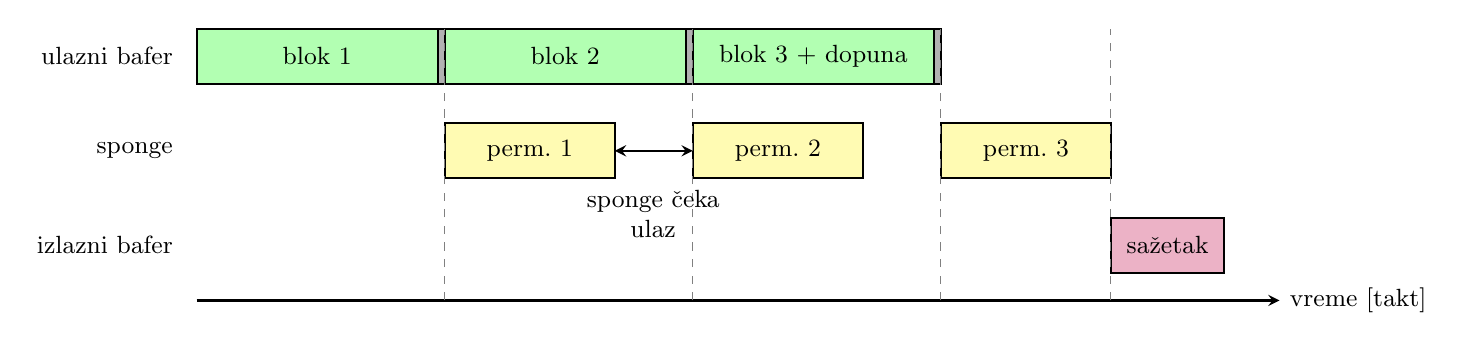
\begin{tikzpicture}[x=0.36cm, y=1cm]
    \draw [thick, ->, >=stealth] (0,-0.7) -- (38.2,-0.7) node[right, font=\small] {vreme [takt]};
    \node [left, font=\small] at (-0.5,2.4) {ulazni bafer};
    \node [left, font=\small] at (-0.5,1.2) {sponge};
    \node [left, font=\small] at (-0.5,0) {izlazni bafer};
    \draw [fill=green!30, thick] (0,2.05) rectangle node[font=\small] {blok 1} (8.5,2.75);
    \draw [fill=gray!60, thick] (8.5,2.05) rectangle (8.75,2.75);
    \draw [fill=green!30, thick] (8.75,2.05) rectangle node[font=\small] {blok 2} (17.25,2.75);
    \draw [fill=gray!60, thick] (17.25,2.05) rectangle (17.5,2.75);
    \draw [fill=green!30, thick] (17.5,2.05) rectangle node[font=\small] {blok 3 + dopuna} (26,2.75);
    \draw [fill=gray!60, thick] (26,2.05) rectangle (26.25,2.75);
    \draw [fill=yellow!30, thick] (8.75,0.85) rectangle node[font=\small] {perm.\ 1} (14.75,1.55);
    \draw [fill=yellow!30, thick] (17.5,0.85) rectangle node[font=\small] {perm.\ 2} (23.5,1.55);
    \draw [fill=yellow!30, thick] (26.25,0.85) rectangle node[font=\small] {perm.\ 3} (32.25,1.55);
    \draw [fill=purple!30, thick] (32.25,-0.35) rectangle node[font=\small] {sažetak} (36.25,0.35);
    \foreach \x in {8.75,17.5,26.25,32.25} { \draw [dashed, gray] (\x,-0.7) -- (\x,2.75); }
    \draw [thick, <->, >=stealth] (14.75,1.2) -- (17.5,1.2);
    \node [font=\small, align=center] at (16.1,0.4) {sponge čeka\\ ulaz};
\end{tikzpicture}
}
\caption{Preklapanje rada stepena za SHA3-256 uz \texttt{DATA\_WIDTH} = 32, gde 34 ulazne reči i takt predaje bloka (uski tamni segment) stoje prema 24 takta permutacije}
\label{fig:sha3_preklapanje}
\end{figure}

Jezgro je u potpunosti parametrizovano genericima, datim u tabeli \ref{tab:sha3_generici}. Jedan isti RTL opis daje svih šest funkcija standarda i cSHAKE konfiguraciju, kako svojstvo iz odeljka \ref{subsec:sha3_varijante} i obećava. Izbor varijante svodi se na raspodelu stanja sponge konstrukcije ($rate = 1600 - 2d$ za SHA3-$d$, a 1344, odnosno 1088, za SHAKE128/256) i bajt dopune. Širina interfejsa \texttt{DATA\_WIDTH} mora deliti i $rate$ i veličinu izlaza, kombinacije koje to ne ispunjavaju odbijaju se pri elaboraciji.

\begin{table}[H]
\caption{Generici SHA-3 akceleratora}
\centering
\resizebox{\textwidth}{!}{
\begin{tabular}{|c|c|c|}
\hline
\rowcolor{gray!30}
Generik & Vrednosti & Uloga \\
\hline
\texttt{ALGORITHM} & \texttt{"SHA3"} / \texttt{"SHAKE"} / \texttt{"CSHAKE"} & familija funkcija i bajt dopune (\texttt{06}/\texttt{1F}/\texttt{04}) \\
\hline
\texttt{SHA3\_VERSION} & \texttt{"224"} / \texttt{"256"} / \texttt{"384"} / \texttt{"512"} & dužina sažetka $d$, odakle je $rate = 1600 - 2d$ \\
\hline
\texttt{SHAKE\_VERSION} & \texttt{"128"} / \texttt{"256"} & $rate$ = 1344 / 1088 \\
\hline
\texttt{SHAKE\_BITS} & umnožak \texttt{DATA\_WIDTH} & ukupna dužina XOF izlaza \\
\hline
\texttt{DATA\_WIDTH} & 8 / 16 / 32 / 64 & širina AXI4-Stream reči \\
\hline
\texttt{ROUNDS\_PER\_CYCLE} & delilac broja 24 & broj rundi permutacije po taktu \\
\hline
\end{tabular}
}
\label{tab:sha3_generici}
\end{table}

\subsection{Ulazni bafer i dopuna}
\label{subsec:hw_sha3_ib}

Ulazni bafer akumulira pristigle reči u registar bloka od $rate$ bitova i vodi računa o dopuni poruke. Modul je realizovan mašinom stanja sa četiri stanja: \texttt{S\_INIT} (početno stanje), \texttt{S\_FILL} (punjenje bloka), \texttt{S\_SEND} (predaja bloka sponge kontroleru) i \texttt{S\_PAD\_BLOCK} (generisanje bloka koji sadrži samo dopunu). Ulaz \texttt{i\_config} je signal omogućavanja jezgra. U trenutnoj realizaciji, gde je varijanta algoritma fiksirana genericima pri sintezi, u AXIS omotaču je vezan na jedinicu, pa jezgro napušta \texttt{S\_INIT} odmah po resetu. Kada stigne reč sa aktivnim \texttt{tlast}, bafer u jednom taktu iznova sastavi reč u kojoj se poruka završava, sa nulama na mestima bajtova koje \texttt{tkeep} maskira i bajtom dopune (\texttt{06} za SHA3, \texttt{1F} za SHAKE, \texttt{04} za cSHAKE) iza poslednjeg važećeg bajta, a kada je poslednja reč poruke puna, bajt dopune otvara narednu reč bloka. Završnu jedinicu šeme bafer postavi zasebnim upisom najvišeg bita bloka, što je tačno dopuna \eqref{eq:sha3_dopuna} iz odeljka \ref{subsec:sha3_dopuna}, sa bitovima razdvajanja domena. Dva granična slučaja zaslužuju pažnju:
\begin{itemize}[itemsep=2pt]
    \item ako dopuna pada na poslednji bajt bloka, bajt dopune i završni bit se stapaju u jedan bajt (\texttt{86}, \texttt{9F}, odnosno \texttt{84}), kako standard i propisuje;
    \item ako se poruka završi tačno na granici bloka, dopuna nema gde da stane, pa se generiše poseban blok koji sadrži samo dopunu (\texttt{S\_PAD\_BLOCK}).
\end{itemize}
\smallbreak
Od organizacije registra bloka neposredno je zavisilo zauzeće ulaznog bafera. Blok se ne drži kao jedan vektor od $rate$ bitova, nego kao niz reči širine \texttt{DATA\_WIDTH}, a svaki upis, bilo da nosi podatak ili dopunu, prolazi kroz jedan jedini upisni port, adresiran rednim brojem reči. Dopuna zauzima jedan dodatni takt, u kome bafer ne prima novu reč. Kroz isti port se tada prepravi tačno jedna reč bloka, a završna jedinica šeme postavlja se zasebnim upisom najvišeg bita bloka. Ovakva organizacija izabrana je zato što se pozicija upisa ne zna unapred, jer zavisi od toga koliko je reči već primljeno i koliko je bajtova poslednje reči maskirano, pa dopuna može početi na bilo kom bajtu bloka.
\smallbreak
Opiše li se takav upis nad jednim širokim vektorom, pozicija se računa u bitovima, izrazom oblika $w \cdot \texttt{DATA\_WIDTH} - m \cdot 8$, koji nije poravnat na granicu reči, pa dekodovanje mora biti u stanju da pogodi bilo koji bajt bloka. Uz to je i širina isečka kojim se brišu maskirani bajtovi promenljiva, što traži generator maske preko celog bloka. Dekoder i izbor po bajtu tada obuhvataju svih $rate/8$ bajtova odjednom, pa je takav opis samo u ulaznom baferu koštao preko 4600 LUT-ova.
\smallbreak
Adresiranje po rečima isti posao svodi na dekoder $1$ od $rate/\texttt{DATA\_WIDTH}$, a izbor između bajta poruke, bajta dopune i nule, koji i dalje zavisi od \texttt{tkeep} signala, ostaje zatvoren unutar jedne reči i svodi se na multiplekser po bajtu. Bajt dopune se pri tome ne upisuje u već sklopljeni blok, nego se cela reč iznova sastavi iz zasebnog registra koji čuva poslednju primljenu reč, čime se izbegava povratna sprega sa registra bloka na samog sebe. Opseg posla time je sveden sa celog bloka na jednu reč, a zauzeće ulaznog bafera na 865 LUT-ova.
\smallbreak
U gustom saobraćaju upravljanje tokom ostaje bezbedno. U taktu u kome se u već pun blok upisuje dopuna, \texttt{tready} je spušten, pa ni paketi koji stižu bez razmaka (novi paket odmah po \texttt{tlast} prethodnog) ne mogu pregaziti blok u pripremi, svojstvo dokazano namenskim testom. Kompletna mašina stanja ulaznog bafera prikazana je na slici \ref{fig:sha3_ib_fsm}.

\begin{figure}[H]
\centering
\resizebox{0.95\textwidth}{!}{
\begin{tikzpicture}[fsm]
    \node [state, initial left] (init) at (0,0) {S\_INIT};
    \node [state] (fill) at (4.8,0) {S\_FILL};
    \node [state] (send) at (9.6,0) {S\_SEND};
    \node [state, font=\footnotesize\ttfamily] (padb) at (9.6,-3.8) {S\_PAD\_BLOCK};
    \path (init) edge node {\texttt{i\_config}} (fill)
          (fill) edge [bend left=18] node {blok spreman} (send)
          (send) edge [bend left=18] node {predat; ima još} (fill)
          (send) edge [bend right=48] node[swap] {predat; kraj poruke} (init)
          (send) edge [bend left=18] node {predat; treba dopuna} (padb)
          (padb) edge [bend left=18] (send);
\end{tikzpicture}
}
\caption{Mašina stanja ulaznog bafera SHA-3 akceleratora}
\label{fig:sha3_ib_fsm}
\end{figure}

\subsection{Sponge kontroler i Keccak jezgro}
\label{subsec:hw_sha3_sponge}

Srce akceleratora je sponge kontroler. Stanje od 1600 bitova drži se u registru. Pri prihvatanju bloka prvih $rate$ bitova stanja sabira se sa blokom (upijanje), a zatim mašina stanja (\texttt{S\_ROUND}) pokreće permutaciju. Tok podataka Keccak jezgra, za obe realizovane arhitekture, prikazan je na slici \ref{fig:sha3_dve_real} u odeljku \ref{subsec:hw_sha3_dve}. Svih pet koraka jedne runde ($\theta$, $\rho$, $\pi$, $\chi$, $\iota$) realizovano je kao čiste funkcije u zajedničkom paketu (\texttt{keccak\_pkg}), pa je runda kombinaciona mreža bez ijednog registra, registruje se samo stanje između taktova. Generik \texttt{ROUNDS\_PER\_CYCLE} određuje koliko se takvih mreža veže u lanac unutar jednog takta, pa stanje \texttt{S\_ROUND} traje onoliko taktova koliko treba da se izvrše sve 24 runde. Kako taj izbor rađa dve arhitekture jezgra pokazuje odeljak \ref{subsec:hw_sha3_dve}. Konstante rundi uzimaju se iz tabele u paketu (dodatak \ref{app:keccak}).

Kontrolerom upravlja mašina stanja prikazana na slici \ref{fig:sha3_sponge_fsm}. U stanju \texttt{S\_ROUND} teče permutacija, u \texttt{S\_WAIT} kontroler čeka naredni blok poruke, a u \texttt{S\_SQUEEZE} nudi isceđeni chunk izlaznom baferu. U stanju \texttt{S\_INIT} prvi blok nove poruke upija se u eksplicitno nulovan registar, jer pri gustom saobraćaju, kada nova poruka stigne odmah po prethodnoj, u registru još stoji zatečena vrednost sa kraja prethodne poruke, a upijanje u nju umesto u nule iskvarilo bi sažetak. I ovaj granični slučaj pokriven je testovima gustog saobraćaja.

\begin{figure}[H]
\centering
\resizebox{0.95\textwidth}{!}{
\begin{tikzpicture}[fsm]
    \node [state, initial left] (init) at (0,0) {S\_INIT};
    \node [state] (round) at (5,0) {S\_ROUND};
    \node [state] (wait) at (5,3.6) {S\_WAIT};
    \node [state, font=\footnotesize\ttfamily] (sqz) at (10.4,0) {S\_SQUEEZE};
    \path (init) edge node {blok} (round)
          (round) edge [bend left=18] node[left=2pt] {kraj perm.; ima još} (wait)
          (wait) edge [bend left=18] node[right=2pt] {novi blok} (round)
          (round) edge [bend left=18] node[above] {kraj perm.; poslednji} (sqz)
          (sqz) edge [bend left=18] node[below, align=center, fill=white, inner sep=2pt] {chunk predat;\\ ima još} (round)
          (sqz) edge [bend left=45] node {chunk predat; kraj} (init);
\end{tikzpicture}
}
\caption{Mašina stanja sponge kontrolera}
\label{fig:sha3_sponge_fsm}
\end{figure}

Za XOF funkcije, kod kojih izlaz premašuje $rate$, kontroler posle predaje svakog chunk-a ponovo permutuje stanje (\texttt{S\_SQUEEZE} $\to$ \texttt{S\_ROUND}). Naredni chunk se pritom permutuje dok izlazni bafer još serijalizuje prethodni, pa dugi XOF izlazi ne unose prazan hod kad god chunk ima bar onoliko reči koliko permutacija traje taktova, resursi ne rastu sa dužinom izlaza, samo latencija (jedna permutacija po chunk-u).

\subsection{Dve realizacije jezgra}
\label{subsec:hw_sha3_dve}

Izbor mikroarhitekture jezgra zasnovan je na analizi prostora arhitektura SHA-3 algoritma koju su dali Sundal i Chaves \cite{sundal_chaves}. Potpuno protočne (engl. \textit{unrolled/pipelined}) arhitekture ostvaruju gotovo jedan sažetak po taktu tek kada se protočni registri popune, što donosi dobit samo kod mnoštva kratkih, međusobno nezavisnih poruka. Nijedna upotreba jezgra u ovom radu ne izgleda tako. Poruka se prima kao jedan tok, pa naredni blok ionako mora sačekati svih 24 runde nad prethodnim i protočnost ne pomaže, a pri izvođenju ključeva, ulozi koju jezgro ima u sistemu, obrađuje se jedna kratka poruka po sesiji. Suprotan pristup, \textit{folded} arhitekture koje po taktu obrađuju samo deo stanja, smanjuje širinu puta podataka, ali usporava sistem približno četiri puta uz nesrazmerno malu uštedu površine zbog dodatne upravljačke logike \cite{sundal_chaves}. Zato je odabrano iterativno jezgro nad celim stanjem. Svih 1600 bitova obrađuje se paralelno, a runde se izvršavaju jedna po taktu, ili dve. Generik \texttt{ROUNDS\_PER\_CYCLE}, broj rundi po taktu (dalje $\mathrm{RPC}$), time postaje osnova dve zasebno sintetisane i ispitane arhitekture, prikazane na slici \ref{fig:sha3_dve_real}:
\begin{itemize}[itemsep=2pt]
    \item \textit{Arhitektura I} ($\mathrm{RPC}=1$) -- jedna kombinaciona runda u povratnoj petlji. Permutacija traje 24 takta, ali je kritična putanja najkraća moguća, dubina jedne runde ($\theta$ do $\iota$);
    \item \textit{Arhitektura II} ($\mathrm{RPC}=2$) -- dve runde vezane u lanac unutar istog takta. Permutacija traje 12 taktova, po cenu približno dvostruko duže kritične putanje i dvostruke količine kombinacione logike.
\end{itemize}

\begin{figure}[H]
\centering
\resizebox{0.95\textwidth}{!}{
\begin{tikzpicture}
    % ================= Arhitektura I =================
    \node (blok1) [blokdata, minimum width=2.2cm, align=center] at (0,4.4) {blok\\ ($rate$ b)};
    \node (xor1) [circle, draw=black, thick, inner sep=2pt] at (1.3,3.1) {$\oplus$};
    % mux
    \draw [thick, fill=gray!15] (0.2,2.3) -- (2.4,2.3) -- (1.95,1.55) -- (0.65,1.55) -- cycle;
    \node [font=\small] at (0.75,2.05) {0};
    \node [font=\small] at (1.85,2.05) {1};
    \node (reg1) [blokdata, minimum width=2.9cm, align=center] at (1.3,0.5) {REG stanja\\ (1600 b)};
    \node (f1) [blokkripto, minimum width=2cm] at (1.3,-1.2) {$f$ (runda)};
    \node (chunk1) [blokrezultat, minimum width=2cm, align=center] at (-1.9,0.5) {chunk\\ izlaza};
    \draw [strelica] (blok1) -| (xor1);
    \draw [strelica] (xor1) -- (0.9,2.3);
    \draw [strelica] (1.3,1.55) -- (reg1);
    \draw [strelica] (reg1) -- (f1);
    \draw [strelica] (reg1) -- (chunk1);
    % povratna petlja
    \draw [thick] (f1.east) -- (3.9,-1.2) -- (3.9,2.7);
    \draw [strelica] (3.9,2.7) -- (1.75,2.7) -- (1.75,2.3);
    \draw [thick] ([yshift=0.3cm]reg1.west) -- (-0.6,0.8) -- (-0.6,3.1);
    \draw [strelica] (-0.6,3.1) -- (xor1);
    \node [right, font=\small] at (3.95,0.9) {$\times 24$};
    \node [font=\small\bfseries, align=center] at (1.3,-2.5) {(a) Arhitektura I: $\mathrm{RPC}=1$\\ \mdseries jedna runda po taktu, 24 takta};
    % ================= Arhitektura II =================
    \node (blok2) [blokdata, minimum width=2.2cm, align=center] at (9,4.4) {blok\\ ($rate$ b)};
    \node (xor2) [circle, draw=black, thick, inner sep=2pt] at (10.3,3.1) {$\oplus$};
    \draw [thick, fill=gray!15] (9.2,2.3) -- (11.4,2.3) -- (10.95,1.55) -- (9.65,1.55) -- cycle;
    \node [font=\small] at (9.75,2.05) {0};
    \node [font=\small] at (10.85,2.05) {1};
    \node (reg2) [blokdata, minimum width=2.9cm, align=center] at (10.3,0.5) {REG stanja\\ (1600 b)};
    \node (f2a) [blokkripto, minimum width=2cm] at (10.3,-1.2) {$f$ (runda)};
    \node (f2b) [blokkripto, minimum width=2cm] at (10.3,-2.7) {$f$ (runda)};
    \node (chunk2) [blokrezultat, minimum width=2cm, align=center] at (7.1,0.5) {chunk\\ izlaza};
    \draw [strelica] (blok2) -| (xor2);
    \draw [strelica] (xor2) -- (9.9,2.3);
    \draw [strelica] (10.3,1.55) -- (reg2);
    \draw [strelica] (reg2) -- (f2a);
    \draw [strelica] (f2a) -- (f2b);
    \draw [strelica] (reg2) -- (chunk2);
    \draw [thick] (f2b.east) -- (12.9,-2.7) -- (12.9,2.7);
    \draw [strelica] (12.9,2.7) -- (10.75,2.7) -- (10.75,2.3);
    \draw [thick] ([yshift=0.3cm]reg2.west) -- (8.4,0.8) -- (8.4,3.1);
    \draw [strelica] (8.4,3.1) -- (xor2);
    \node [right, font=\small] at (12.95,0.9) {$\times 12$};
    \node [font=\small\bfseries, align=center] at (10.3,-3.9) {(b) Arhitektura II: $\mathrm{RPC}=2$\\ \mdseries dve runde po taktu, 12 taktova};
\end{tikzpicture}
}
\caption[Tok podataka Keccak jezgra za obe arhitekture]{Tok podataka Keccak jezgra za obe arhitekture, prilagođeno prema \cite{sundal_chaves}. Multiplekser bira između upijanja novog bloka (ulaz 0, blok sabran sa registrovanim stanjem, kod prvog bloka poruke nultim) i rezultata rundi (ulaz 1). (a) jedna runda po taktu, (b) dve vezane runde po taktu}
\label{fig:sha3_dve_real}
\end{figure}

Arhitektura II na prvi pogled nudi dvostruku propusnost, ali kompromis ima dva ograničenja. Prvo, duža kritična putanja obara radnu učestanost, pa deo dobitka u taktovima poništi produženi period, a vrednosti generika iznad 2 iz istog razloga očekivano daju sve manji dobitak, jer putanja raste brže nego što broj taktova opada. Koliko učestanost zaista pada izmereno je u odeljku \ref{subsec:rez_sha3_resursi}. Drugo, kod konfiguracija kod kojih punjenje bloka traje duže od permutacije (\texttt{DATA\_WIDTH} znatno manji od $rate$), skraćenje permutacije ne menja ništa, jer jezgro ionako čeka ulaz. Zbog toga su obe arhitekture izmerene nad svih sedam kombinacija varijante i širine koje elaboracija dopušta, ukupno četrnaest konfiguracija (odeljak \ref{subsec:rez_sha3_resursi}).

\subsection{Izlazni bafer}
\label{subsec:hw_sha3_ob}

Izlazni bafer prihvata chunk od sponge kontrolera i serijalizuje ga u \texttt{DATA\_WIDTH} reči na master AXI4-Stream interfejsu, uz \texttt{tlast} na poslednjoj reči ukupnog izlaza. Bafer drži sopstvenu kopiju chunk-a, pa se iznošenje tekućeg preklapa sa računanjem narednog u kontroleru, a chunk koji stigne na vreme nadovezuje se bez praznog takta između reči. Svaka reč, uključujući poslednju, ostaje validna dok je \texttt{tready} ne prihvati, pa je izlaz bezbedan i pod proizvoljnim protivpritiskom potrošača.

\subsection{Podrška za cSHAKE i KMAC}
\label{subsec:hw_sha3_kmac}

Odeljak \ref{subsec:kmac} pokazao je da je celokupno KMAC uokvirivanje samo formatiranje ulaznog niza, u kome se prefiksni blok sa imenom funkcije, blok ključa i kodirana dužina izlaza redom nadovezuju pre poruke.
\smallbreak
Iz toga sledi da KMAC nema svoj režim u hardveru. Jezgro realizuje samo cSHAKE, a od funkcije SHAKE ga razlikuje jedino bajt dopune, koji konfiguracija \texttt{ALGORITHM = "CSHAKE"} postavlja na \texttt{04} umesto na \texttt{1F}. Pošto je izbor utvrđen generikom, jezgro za prazne $N$ i $S$ ne prelazi u SHAKE, kako standard za taj slučaj propisuje, i tu se od njega razilazi. Sve ostalo stiže kao obična poruka, čiji sastav jezgro ne proverava. Uokvirivanje je time ostavljeno strani koja podatke dovodi, na kojoj je i obaveza da režim koristi sa nepraznim prefiksnim blokom, kod KMAC-a uvek ispunjena, jer ime funkcije propisuje sam standard (odeljak \ref{subsec:kmac}). U proveri iz ovog rada to je referentni model, dok bi u sistemu jednako poslužio upravljački program ili jednostavan upravljački blok ispred jezgra.
\smallbreak
Podela je proverena namenskim testom sa poznatim odgovorima, nad KMAC256 i KMACXOF256 vektorima koje je proizveo referentni model, program u jeziku Python koji iste funkcije izračunava nezavisno od jezgra i sam je prethodno upoređen sa standardnom bibliotekom (odeljak \ref{sec:rez_metodologija}).

\subsection{Uklapanje u sistem i provera}
\label{subsec:hw_sha3_uklapanje}

Jezgro je projektovano kao koprocesor iza kontrolera za neposredan pristup memoriji (engl. \textit{Direct Memory Access}, DMA). Procesorski sistem preda poruku u memoriju, DMA je propusti kroz jezgro, a sažetak se vrati u memoriju. Takva postavka odgovara grupnom heširanju, kod koga je merilo propusnost nad dugom porukom, dok je za izvođenje ključeva merodavna latencija kratke poruke, izmerena u odeljku \ref{subsec:rez_sha3_propusnost}. Koja veličina postavlja granicu propusnosti za svaku konfiguraciju, i gde udvostručenje broja rundi po taktu ima smisla, pokazuje model uskog grla iz istog odeljka.
\smallbreak
Jezgro pritom nije vezano za ulogu u lancu, pa jednako služi za opšte heširanje podataka i kao izvor pseudoslučajnog niza proizvoljne dužine.
\smallbreak
Jezgro je provereno na tri nivoa, od vektora sa poznatim odgovorima do rada na ploči. Postupci i svi rezultati dati su u odeljku \ref{sec:rez_sha3}.

\section{AES-GCM akcelerator}
\label{sec:hw_aesgcm}

\subsection{Organizacija akceleratora}
\label{subsec:hw_gcm_pregled}

AES-GCM akcelerator projektovan je kao umetnuta zaštita paketa. Paket uđe u jezgro i isti taj paket izađe, sa zaštićenim korisnim sadržajem i nepromenjenim zaglavljima. To ga razlikuje od SHA-3 jezgra, koje poruku potroši i vrati sažetak. Ovde ulaz i izlaz imaju istu strukturu, pa jezgro može stajati usred puta kojim paket ionako prolazi. Paket se posmatra kao niz segmenata, datih u tabeli \ref{tab:gcm_segmenti}.

\begin{table}[H]
\caption{Segmenti paketa u AES-GCM akceleratoru}
\centering
\resizebox{\textwidth}{!}{
\begin{tabular}{|c|c|}
\hline
\rowcolor{gray!30}
Segment & Uloga \\
\hline
BYPASS & Prenosi se nepromenjen, mimo kriptografskog puta (npr.\ zaglavlja nižih slojeva). \\
\hline
AAD & Autentifikuje se, ali se ne šifruje, pa ulazi u GHASH i izlazi nepromenjen. \\
\hline
PT / CT & Korisni sadržaj, koji se i šifruje i autentifikuje. Dužina se otkriva u radu, iz \texttt{tlast}. \\
\hline
ICV & Autentifikaciona oznaka od 16 bajtova. Dodaje se pri šifrovanju, proverava pri dešifrovanju. \\
\hline
\end{tabular}
}
\label{tab:gcm_segmenti}
\end{table}

Šifrovanje time preslikava \mbox{$\mathrm{BYPASS} \,\|\, \mathrm{AAD} \,\|\, \mathrm{PT}$} u \mbox{$\mathrm{BYPASS} \,\|\, \mathrm{AAD} \,\|\, \mathrm{CT} \,\|\, \mathrm{ICV}$}, a dešifrovanje obrnuto, uz dodatni izlazni signal koji govori da li je oznaka ispravna. Dužine segmenata BYPASS i AAD zadaju se generički, dok se dužina korisnog sadržaja ne zna unapred.
\smallbreak
Akcelerator je izgrađen od tri sloja, koji odgovaraju i podeli na IP jezgra:
\begin{enumerate}[itemsep=2pt]
    \item \textit{Kriptografsko jezgro} (\texttt{AES\_algorithm}) -- sama šifra;
    \item \textit{GCM sloj} (\texttt{gcm\_enc\_glue}, \texttt{gcm\_dec\_glue}) -- sve ostalo iz GCM režima: GHASH, blok sa dužinama, formiranje i provera oznake;
    \item \textit{Sistemski omotač} -- razdvajanje i ponovno sastavljanje segmenata stvarnog paketa.
\end{enumerate}
Granica između prvog i drugog sloja namerno je postavljena kao fiksna lista portova. Sloj ne zna koju šifru vodi, a jezgro ne zna kojim smerom sloj radi, jer je XOR sam sebi inverzan, pa ista instanca jezgra stoji i na putu šifrovanja i na putu dešifrovanja. GCM režim je pritom ugrađen u samo jezgro, koje formira brojački blok i računa potključ $H$ i masku oznake. Ta granica je i osnova za dinamičku rekonfiguraciju, o čemu je reč u odeljku \ref{subsec:hw_dfx}.

\subsection{AES jezgro}
\label{subsec:hw_aes_jezgro}

\subsubsection{Šta jezgro računa}

Iz opisa GCM režima (odeljak \ref{subsec:gcm_rezim}) sledi da su jezgru potrebne tri vrste blokova:
\begin{enumerate}[itemsep=2pt]
    \item $H = E_K(0^{128})$ -- heš potključ za GHASH. Zavisi samo od ključa, pa se računa jednom po ključu i izlazi bočnim kanalom;
    \item $E_K(J_0)$ -- maska autentifikacione oznake. Zavisi od nonce vrednosti, pa se računa jednom po paketu, takođe bočnim kanalom;
    \item $E_K(J_0+1), E_K(J_0+2), \ldots$ -- niz koji se sabira sa korisnim sadržajem, jedan blok po bloku podataka.
\end{enumerate}
Sve tri su obična šifrovanja jednog bloka. Blok šifra se nikada ne invertuje, pa jezgro ne sadrži nijednu inverznu transformaciju, isti modul, bez ijedne izmene, koristi se i na putu šifrovanja i na putu dešifrovanja, što je već najavljeno u odeljku \ref{subsec:aes_dekripcija}. Kroz samu šifru pritom prolaze isključivo ovi blokovi, dok se korisni sadržaj sa nizom sabira tek na izlazu omotača i u jezgro nikada ne ulazi.
\smallbreak
Brojački blok se formira u hardveru. Iz 96-bitnog ulaza \texttt{i\_nonce} gradi se $J_0 = \mathit{nonce} \,\|\, 0^{31} \,\|\, 1$, a dalji blokovi inkrementiranjem donjih 32 bita, dok gornjih 96 ostaje zaključano. Onaj ko jezgro pokreće bira, dakle, samo nonce, a ne i sam brojač, pa se brojački blokovi unutar paketa ne mogu ni ponoviti ni preskočiti. Ponavljanje niza između paketa svodi se time na ponavljanje nonce vrednosti, o čijoj je dodeli reč u odeljku \ref{subsec:gcm_sigurnost}. Ovakav sastav nonce vrednosti poklapa se sa načinom na koji je definišu IPsec \cite{rfc4106} i MACsec, kod kojih jedan deo nonce vrednosti ostaje isti tokom čitavog trajanja veze, a ostatak je brojač paketa.

\subsubsection{Dve arhitekture jezgra}
\label{subsec:hw_aes_arh}

Kao i kod SHA-3 jezgra, ista funkcionalnost realizovana je u dve arhitekture, koje se biraju generikom \texttt{WRAPPER\_KIND}.
\smallbreak
\textit{Protočna arhitektura} (\texttt{UNROLLED}) sadrži jedno potpuno protočno AES jezgro dubine $N_r + 2$ stepena, koje u ustaljenom stanju daje jedan blok po taktu.
\smallbreak
Rundi ima $N_r$, a stepena dva više. Prvi dodatni je početno sabiranje sa ključem, registrovano kao i svaki drugi stepen. Drugi je stepen koji se sastoji samo od registra, umetnut neposredno pred poslednju rundu. On postoji zbog spoja koji se javlja samo na tom mestu. Poslednja runda nema MixColumns, pa se jedina uvek realizuje kombinacionom logikom (odeljak \ref{subsec:hw_aes_round_style}), a kod BRAM stila ispred nje stoji izlaz memorije sa T-tabelama, osetno sporiji od izlaza običnog registra. Bez ovog stepena izlaz memorije, XOR sloj runde i cela logika poslednje runde našli bi se na istoj putanji, koja ne ispunjava vremenske uslove. Registar je seče na dva kratka takta. Kod LUT stila takve putanje nema, pa je tamo ovaj stepen samo cena uniformnosti, 128 flip-flopova i jedan takt latencije, kojom dubina protoka i upravljačka logika ostaju iste za oba stila.
\smallbreak
Kroz taj isti protok prolaze tri vrste blokova, i to bez ikakvog razdvajanja u faze. Raspoređivač (engl. \textit{dispatcher}) ih propušta jedan za drugim, a svakom pridružuje dvobitnu oznaku uloge koja putuje uz podatak, u korisničkom signalu \texttt{tuser} AXI4-Stream interfejsa. Na izlazu demultiplekser po njoj usmerava blok, u registar za $H$, u registar za masku oznake, ili u XOR sa korisnim sadržajem, dok je protok samo prenosi, ne ispitujući je. Postupak je prikazan na slici \ref{fig:aes_unrolled}.

\begin{figure}[H]
\centering
\resizebox{\textwidth}{!}{
\begin{tikzpicture}[font=\large, >=stealth]
    % --- ulazni blokovi i raspoređivač ---
    \node (disp) [blokkripto, minimum width=2.2cm, minimum height=4.0cm, align=center] at (0,0)
        {raspo-\\ređivač};
    \node (b1) [blokdata, minimum width=1.8cm, minimum height=0.9cm] at (-3.0, 1.7) {$0^{128}$};
    \node (b2) [blokdata, minimum width=1.8cm, minimum height=0.9cm] at (-3.0, 0.0) {$J_0$};
    \node (b3) [blokdata, minimum width=1.8cm, minimum height=0.9cm] at (-3.0,-1.7) {$CB_i$};
    \foreach \i in {1,2,3} { \draw [strelica] (b\i) -- (b\i -| disp.west); }

    % --- protok ---
    \foreach \i/\x/\lab in {1/2.9/{sabiranje\\ sa $K_0$}, 2/5.2/{runda 1},
                            4/11.3/{runda $N_r$}} {
        \node (s\i) [blokkripto, minimum width=1.9cm, minimum height=2.0cm, align=center] at (\x,0) {\lab};
        \fill [black!60] ([xshift=-0.16cm, yshift=-0.07cm]s\i.north east) rectangle ([yshift=0.07cm]s\i.south east);
    }
    \node (s3) [draw=black, fill=black!60, minimum width=0.3cm, minimum height=2.0cm, inner sep=0pt] at (9.0,0) {};
    \node [below=0.05cm of s3, font=\small] {registar};
    \node at (7.1,0) {\Huge $\cdots$};
    \draw [strelica] (disp.east) -- (s1);
    \draw [strelica] (s1) -- (s2);
    \draw [strelica] (s2) -- (6.5,0);
    \draw [strelica] (7.7,0) -- (s3);
    \draw [strelica] (s3) -- (s4);

    % --- tuser kanal, iznad protoka ---
    \draw [strelica, dashed, gray!70, thick] (0,2.1) -- (0,3.5) -- (13.9,3.5) -- (13.9,2.1);
    \node [gray!60!black] at (7.0,3.9) {oznaka uloge bloka putuje kroz \texttt{tuser}, uz podatak};

    % --- demultiplekser i tri odredišta ---
    \node (dmx) [blokghash, minimum width=2.2cm, minimum height=4.0cm, align=center] at (13.9,0)
        {demulti-\\plekser};
    \draw [strelica] (s4) -- (dmx);
    \node (d1) [blokrezultat, minimum width=3.6cm, minimum height=0.9cm] at (17.9, 1.7) {registar za $H$};
    \node (d2) [blokrezultat, minimum width=3.6cm, minimum height=0.9cm] at (17.9, 0.0) {maska oznake};
    \node (d3) [blokrezultat, minimum width=3.6cm, minimum height=0.9cm] at (17.9,-1.7) {XOR sa sadržajem};
    \foreach \i in {1,2,3} { \draw [strelica] (d\i -| dmx.east) -- (d\i); }

    % --- okvir protoka ---
    \node [draw=black, dashed, thick, inner sep=0.4cm, fit=(s1)(s4),
           label={[font=\large, yshift=-0.45cm]below:{protok dubine $N_r + 2$ stepena, jedan blok po taktu}}] {};
\end{tikzpicture}
}
\caption[Protočna arhitektura AES jezgra]{Protočna arhitektura AES jezgra. Svaki stepen protoka završava se svojim registrom (tamna traka uz desnu ivicu), a stepen registar sastoji se samo od njega}
\label{fig:aes_unrolled}
\end{figure}

\smallbreak
\textit{Višejezgarna arhitektura} (\texttt{MULTICORE}) sadrži \texttt{NUM\_CORES} iterativnih jezgara. Jezgro računa blok $N_r$ taktova, a zatim rezultat drži još jedan takt na registarskom izlazu, dok ga omotač ne preuzme. Blok, dakle, zauzima jezgro $N_r + 1$ taktova, pa je zbirna propusnost
\begin{equation}
    \label{eq:multicore_propusnost}
    B_{\mathrm{takt}} = \min\!\left(\frac{\texttt{NUM\_CORES}}{N_r + 1},\ 1\right) \ \text{blokova po taktu},
\end{equation}
gde gornju granicu postavlja jedan izlazni port, koji ne može otpustiti više od jednog bloka po taktu. Jedan blok po taktu postiže se, dakle, sa $N_r + 1$ jezgara, što kod AES-256 znači petnaest jezgara. Raspodela posla je kružna (engl. \textit{round-robin}), sa dva nezavisna pokazivača, prikazana na slici \ref{fig:aes_rr}:
\begin{itemize}[itemsep=2pt]
    \item \texttt{r\_start\_onehot} -- koje jezgro sledeće prima blok, napreduje na svako prihvaćeno pokretanje;
    \item \texttt{r\_out\_onehot} -- čiji se rezultat sledeće otpušta, napreduje na svako otpuštanje.
\end{itemize}

\begin{figure}[H]
\centering
\resizebox{0.9\textwidth}{!}{
\begin{tikzpicture}
    \node (disp) [blokkripto, minimum width=2.6cm, minimum height=1.2cm, align=center] at (0,0) {raspodela\\ \texttt{r\_start\_onehot}};
    \node (c0) [blokdata, minimum width=2.2cm] at (4.4,2.4) {jezgro 0};
    \node (c1) [blokdata, minimum width=2.2cm] at (4.4,0.8) {jezgro 1};
    \node (c2) [blokdata, minimum width=2.2cm] at (4.4,-0.8) {jezgro 2};
    \node (c3) [blokdata, minimum width=2.2cm] at (4.4,-2.4) {jezgro 3};
    \node (rel) [blokghash, minimum width=2.6cm, minimum height=1.2cm, align=center] at (8.8,0) {otpuštanje\\ \texttt{r\_out\_onehot}};
    \foreach \c in {c0,c1,c2,c3} {
        \draw [strelica] (disp) -- (\c);
        \draw [strelica] (\c) -- (rel);
    }
    \node [font=\small, align=center] at (0,-2.2) {kreće čim je\\ jezgro slobodno};
    \node [font=\small, align=center] at (8.8,-2.2) {strogo po redosledu\\ raspodele};
\end{tikzpicture}
}
\caption{Kružna raspodela u višejezgarnoj arhitekturi}
\label{fig:aes_rr}
\end{figure}

Dva pokazivača idu nezavisno, oba kružnim redom. Ulazni pokreće naredno jezgro čim je ono prazno, nezavisno od toga dokle je izlazni stigao. Zaustavlja se jedino kad ga sustigne, jer sme da pokrene samo prazno jezgro. Pokretanje pritom ne čeka ni da reč podataka stigne, pa niz nastaje unapred. Izlazni otpušta rezultate strogo redom, jezgro po jezgro, pa jezgro koje završi ranije čeka svoj red. Niz koji na kraju paketa ostane neiskorišćen odbacuje se pri pražnjenju. Oba pokazivača su kružne one-hot dozvole koje se pomeraju na sam događaj, prihvaćeno pokretanje odnosno otpuštenu reč, pa izbor jezgra ne traži dekoder. Uz izlaznu dozvolu napreduje i mali binarni pratilac, koji služi samo kao izbor multipleksera rezultata, jer je za širinu od 128 bitova binarni izbor jeftiniji od one-hot mreže.
\smallbreak
Šta je otpušteni blok, $H$, maska oznake ili niz za šifrovanje, ne pamti se po jezgru, već sledi iz dve zastavice. Dok $H$ za tekući ključ nije zabeležen, prvi gotov rezultat je $H$. Dok maska za tekući paket nije zabeležena, sledeći je maska. Posle toga svi su blokovi niza. Prva dva otpuštaju se bezuslovno, jer ih niko nizvodno ne mora prihvatiti, dok se blok niza otpušta samo uz potpuno rukovanje sa oba kraja.

\subsubsection{Ekspanzija ključa u hodu}
\label{subsec:hw_aes_kljuc}

Ključevi rundi iz odeljka \ref{subsec:aes_ekspanzija} mogu se izračunati unapred i zadržati u registrima, ili generisati u hodu (engl. \textit{on-the-fly}), uporedo sa samim rundama. Ovde je izabrano drugo, a presudan je rad sa više ključeva odjednom. Na primer, čvor koji nosi $N$ IPsec tunela ima po jedan ključ za svaki tunel, i paketi različitih tunela smenjuju se na istom akceleratoru.
\smallbreak
Sa unapred izračunatim ključevima takav rad ostavlja dva loša izbora: ili se pri svakoj promeni ključa čeka nova ekspanzija, pa protok pada, ili se prošireni ključevi keširaju, po 240 bajtova registara za svaki, pa zauzeće raste linearno sa brojem tunela. Generisanje u hodu uklanja oba, jer se za svaki ključ čuva samo polazni oblik, prošireni postoji jedino za ključ u upotrebi, a jedina cena promene ključa je jedno šifrovanje bloka više, kojim se preračunava potključ $H$ za GHASH.
\smallbreak
Sama ekspanzija pritom ne unosi nikakav zastoj. Jezgro nema fazu „proširi ključ, pa počni" niti rukovanje tipa „ključevi spremni". Ekspander proizvodi ključ runde $K_i$ tačno jedan takt pre runde koja ga koristi, u koraku sa jezgrima, pa promena ključa ne košta nijedan prazan paket. Jedino što mora biti usklađeno jeste trenutak prve raspodele, i on kod višejezgarne arhitekture zavisi od dužine ključa. Kod AES-256 su $K_0$ i $K_1$ validni već u drugom ciklusu, dok kod AES-128 $K_1$ postaje validan tek u trećem, pa se prva raspodela zadržava za jedan takt.
\smallbreak
U višejezgarnoj arhitekturi jezgra ključeve rundi ne čitaju iz zajedničkog niza registara. Ekspander ključ svake runde emituje kao upis svim jezgrima, a svako ga upiše u sopstvenu distribuiranu memoriju od šesnaest reči i čita lokalno, po svom brojaču runde. Jezgro tako ne nosi multiplekser za izbor ključa, a raspored ključeva ne putuje preko čipa. Protočna arhitektura, sa jednim protokom, ključeve čita neposredno iz niza ekspandera, svaki stepen ključ svoje runde.
\smallbreak
Poseban problem je ključ ili nonce koji stigne usred paketa. Ključevi rundi se u tom trenutku čitaju, a brojački blok je usred niza, pa ni jedno ni drugo ne sme da se promeni dok paket traje. Jezgro zato za obe vrednosti drži po jedan senka registar (engl. \textit{shadow register}). Pristigla vrednost ne dira aktivnu, nego čeka u senci. Na ciklusu pražnjenja, kada se poslednja reč paketa preda, senka postaje aktivna vrednost, ekspander se pokreće ispočetka, a bočni signal javlja da je $H$ zastareo dok se ne preračuna. Vremenski tok prikazan je na slici \ref{fig:aes_kljuc_nonce}.

\begin{figure}[H]
\centering
\resizebox{\textwidth}{!}{
\begin{tikzpicture}[font=\large, >=stealth,
    sig/.style={anchor=east, font=\large\ttfamily},
    band/.style={draw=black!55, rounded corners=2pt, minimum height=0.9cm, align=center, font=\large}]

    \def\xa{1.0}\def\xb{3.0}\def\xc{5.0}\def\xd{7.0}\def\xe{9.0}\def\xf{11.0}\def\xg{13.0}

    % vremenska osa
    \foreach \x/\t in {\xa/$t_0$, \xb/$t_1$, \xc/$t_2$, \xd/$t_3$, \xe/$t_4$, \xf/$t_5$, \xg/$t_6$} {
        \draw [gray!35] (\x,0.2) -- (\x,7.6);
        \node [font=\small, gray!60!black] at (\x,7.9) {\t};
    }
    \node [font=\small, gray!60!black, anchor=south] at (\xe,8.3) {\texttt{tlast}};
    \node [font=\small, red!60!black, anchor=south] at (\xf,8.9) {pražnjenje};
    \draw [dashed, red!70, thick] (\xf,0.2) -- (\xf,8.9);

    % --- redovi ---
    \node [sig] at (0.6,7.0) {i\_key\_valid};
    \node [sig] at (0.6,6.55) {i\_nonce\_valid};
    \node [band, fill=yellow!30, minimum width=1.6cm] at (\xc,6.8) {impuls\\ $K_2$, $N_2$};

    \node [sig] at (0.6,5.6) {s\_axis (paket A)};
    \node [band, fill=green!30, minimum width=7.4cm] at (5.6,5.6) {reči paketa A, ključ $K_1$, nonce $N_1$};
    \node [band, fill=green!30, minimum width=2.6cm] at (12.5,5.6) {paket B, $K_2$, $N_2$};

    \node [sig] at (0.6,4.6) {r\_active\_key};
    \node [sig] at (0.6,4.15) {r\_active\_IV};
    \node [band, fill=gray!20, minimum width=9.4cm] at (5.9,4.4) {$K_1$, \; $J_0 = N_1 \,\|\, 0^{31}1$, brojač napreduje};
    \node [band, fill=gray!20, minimum width=2.6cm] at (12.5,4.4) {$K_2$, \; $J_0 = N_2 \,\|\, 0^{31}1$};

    \node [sig] at (0.6,3.4) {r\_shadow\_key};
    \node [sig] at (0.6,2.95) {r\_shadow\_IV};
    \node [band, fill=orange!25, minimum width=6.4cm] at (7.8,3.2) {$K_2$, $N_2$ čekaju u senci (paket A još traje)};

    \node [sig] at (0.6,2.0) {KeyExpansion};
    \node [band, fill=cyan!25, minimum width=9.4cm] at (5.9,2.0) {ključevi rundi $K_1$, takt ispred jezgara};
    \node [band, fill=cyan!25, minimum width=2.6cm] at (12.5,2.0) {ključevi rundi $K_2$};

    \node [sig] at (0.6,0.8) {o\_h\_stale};
    \node [band, fill=red!20, minimum width=2.6cm] at (12.5,0.8) {$H$ zastareo};

    % strelica: senka -> aktivno, na praznjenju
    \draw [strelica, orange!80!black, thick] (10.9,3.2) .. controls (11.9,3.2) and (12.4,3.6) .. (12.4,4.85);
\end{tikzpicture}
}
\caption{Ključ i nonce pristigli usred paketa ($t_2$) primenjuju se tek na ciklusu pražnjenja ($t_5$)}
\label{fig:aes_kljuc_nonce}
\end{figure}

Tri pravila pokrivaju granične slučajeve, i sva tri su potvrđena namenskim testovima:
\begin{itemize}[itemsep=2pt]
    \item \textit{poslednji upis važi} -- vrednost koja stigne baš na ciklusu pražnjenja pretiče onu koja već čeka u senci, pa nijedna izmena ne biva tiho izgubljena;
    \item \textit{nezavisno pristizanje} -- nonce pre ključa i ključ bez nonce vrednosti su podjednako dozvoljeni. Paket jednostavno čeka dok oba ne budu na mestu;
    \item \textit{zaštita od ponovne upotrebe} -- ako nijedna nonce vrednost nije u senci, jezgro na kraju paketa zaboravlja tekuću, pa naredni paket ne može krenuti dok se ne dobije sveža. Tiho ponavljanje brojačkog bloka nije dostižno preko interfejsa.
\end{itemize}

\subsubsection{Upravljanje tokom: \texttt{FLOW\_STYLE}}
\label{subsec:hw_aes_flow}

Unutar protočne arhitekture, način na koji se izvode dozvole za pomeranje stepena bira se generikom \texttt{FLOW\_STYLE}. Oba izbora vode isti protok i daju isti šifrat.
\smallbreak
Pre opisa treba uvesti dve veličine na koje se oba načina oslanjaju. \textit{Vektor validnosti} je niz od $N_r + 2$ bita, po jedan za svaki stepen protoka, i bit $i$ kaže da stepen $i$ trenutno drži važeći blok. \textit{Spremnost nizvodne strane} je signal \texttt{m\_axis\_tready}, kojim potrošač na izlazu javlja da može da primi reč. Prazan stepen usred punog protoka naziva se \textit{mehur}. On ne nosi podatak, ali zauzima mesto i putuje kroz protok kao i svaki blok.
\smallbreak
\textit{GLOBAL} izvodi jednu jedinu dozvolu i razvodi je svim stepenima, pa se ceo protok pomera zajedno ili nikako. Dozvola se računa neposredno iz vektora validnosti i signala \texttt{m\_axis\_tready}, bez ijednog pomoćnog registra. Time je vektor validnosti jedini merodavan zapis o tome šta je u protoku, i ne postoji brojač koji bi se mogao raspariti sa stvarnim sadržajem. Mana je što mehur nastao u sredini nikada ne nestaje. Pošto se ceo protok pomera zajedno, prazan stepen putuje sve do izlaza. Zastoj na izlazu, međutim, ne zaustavlja odmah i glavu protoka, jer dozvola ostaje aktivna dok god je poslednji stepen slobodan. Protok, dakle, nastavlja da prima dok se ne popuni, i tek tada staje. Dok stoji, poslednji stepen drži gotov blok sve dok ga potrošač ne primi, pa se pod protivpritiskom nijedan rezultat ne gubi.
\smallbreak
\textit{PER\_STAGE}, preuzet iz \cite{gavrilovic_diplomski}, daje svakom stepenu sopstveni brojač zauzeća i prag koji opada sa indeksom stepena, tako da kasniji stepeni prestaju da primaju pre ranijih. Glava protoka može da nastavi sa punjenjem i pošto se poslednji stepen popuni, jer svaki stepen odlučuje sam za sebe, pa se mehuri istiskuju. Cena su $N_r + 2$ brojača i komparatora, i drugi izvor istine, koji mora ostati usklađen sa vektorom validnosti. Upravo taj problem GLOBAL nema, jer nema ni brojače. Oba načina prikazana su na slici \ref{fig:aes_flow}.

\begin{figure}[H]
\centering
\resizebox{\textwidth}{!}{
\begin{tikzpicture}[font=\large, >=stealth]
    % ---------- GLOBAL ----------
    \begin{scope}
    \node [font=\large\bfseries, anchor=west] at (-1.6,2.2) {(a) \texttt{GLOBAL}};
    \foreach \i/\x in {0/1.6, 1/3.7, 2/5.8, 3/7.9} {
        \node (g\i) [blokkripto, minimum width=1.5cm, minimum height=1.3cm] at (\x,0.8) {$s_\i$};
    }
    \node at (9.6,0.8) {\Large $\cdots$};
    \foreach \i/\j in {0/1, 1/2, 2/3} { \draw [strelica] (g\i) -- (g\j); }
    \draw [strelica] (-0.3,0.8) -- node[above, pos=0.2, font=\small\ttfamily] {s\_axis} (g0);
    \draw [strelica] (10.4,0.8) -- node[above, font=\small\ttfamily] {m\_axis} (11.9,0.8);
    % jedna dozvola za sve
    \node (ge) [blokghash, minimum width=4.6cm, minimum height=0.9cm] at (5.4,-1.5) {jedna dozvola za sve stepene};
    \foreach \i in {0,1,2,3} { \draw [strelica, gray!70] (ge.north) -- (g\i.south); }
    \draw [strelica, red!70] (11.9,0.1) -- (11.9,-1.5) -- node[above, font=\small\ttfamily] {m\_axis\_tready} (ge.east);
    \node [font=\small, align=left, anchor=north west] at (10.6,-2.1) {protok staje tek\\ kada se popuni};
    \end{scope}

    % ---------- PER_STAGE ----------
    \begin{scope}[yshift=-5.4cm]
    \node [font=\large\bfseries, anchor=west] at (-1.6,2.2) {(b) \texttt{PER\_STAGE}};
    \foreach \i/\x in {0/1.6, 1/3.7, 2/5.8, 3/7.9} {
        \node (p\i) [blokkripto, minimum width=1.5cm, minimum height=1.3cm] at (\x,0.8) {$s_\i$};
        \node (c\i) [blokdata, minimum width=1.5cm, minimum height=0.8cm] at (\x,-1.2) {brojač};
        \draw [strelica, gray!70] (c\i) -- (p\i);
    }
    \node at (9.6,0.8) {\Large $\cdots$};
    \foreach \i/\j in {0/1, 1/2, 2/3} { \draw [strelica] (p\i) -- (p\j); }
    \draw [strelica] (-0.3,0.8) -- node[above, pos=0.2, font=\small\ttfamily] {s\_axis} (p0);
    \draw [strelica] (10.4,0.8) -- node[above, font=\small\ttfamily] {m\_axis} (11.9,0.8);
    \draw [strelica, red!70] (11.9,0.1) -- (11.9,-1.2) -- node[above, font=\small\ttfamily] {m\_axis\_tready} (c3.east);
    \node [font=\small, align=left, anchor=north west] at (10.6,-1.8) {glava se puni\\ dok rep stoji};
    \node [font=\small, gray!60!black, anchor=north] at (5.4,-2.0) {prag opada sa indeksom stepena};
    \end{scope}
\end{tikzpicture}
}
\caption{Dva načina upravljanja tokom u protočnoj arhitekturi: (a) jedna zajednička dozvola, pa se protok pomera u celini, a (b) po jedan brojač zauzeća po stepenu, pa glava protoka nastavlja da prima dok rep stoji}
\label{fig:aes_flow}
\end{figure}

U GCM sistemu protok puni jedan raspoređivač, a prazni ga jedan XOR, pa je po pravilu pun i mehuri su retki. Zbog toga je GLOBAL podrazumevani izbor, a poređenje dva stila pod zastojem dato je u odeljku \ref{subsec:rez_aes_protivpritisak}.

\subsubsection{Realizacija runde: \texttt{ROUND\_STYLE}}
\label{subsec:hw_aes_round_style}

Poslednji izbor je kojim resursom se računa runda. Obe varijante imaju isto kašnjenje od jednog takta i daju isti rezultat.
\smallbreak
\textit{BRAM} (engl. \textit{Block RAM}, ugrađeni memorijski blok) koristi T-tabele iz odeljka \ref{subsec:aes_ttabele}, pa runda postaje XOR četiri tabelarna čitanja, čitanje iz memorije umesto aritmetike. Svaka od četiri kolone realizovana je zasebnom instancom koja izvršava četiri čitanja, a ShiftRows je utkan u to koja četiri bajta stanja koja instanca čita, kolona 0 čita bajtove 0, 5, 10 i 15, kolona 1 bajtove 4, 9, 14 i 3, i tako dalje. Tabela se čuva samo jednom, jer se $T_1$, $T_2$ i $T_3$ dobijaju rotacijom pročitane $T_0$ vrednosti, preuređenjem veza posle registra, bez ijednog logičkog elementa. XOR koji spaja četiri rotirane vrednosti i ključ runde ima pet ulaza po bitu, pa staje u jednu šestoulaznu tabelu.
\smallbreak
\textit{LUT} varijanta ispisuje rundu kao lanac četiri transformacije i registruje ga jednom na kraju. Sve završava u logici, S-boks kao kombinaciona mreža, MixColumns kao stabla XOR kola. Nula memorijskih blokova, ali četiri kombinaciona koraka leže u seriji unutar jednog takta, i ta serija je kritična putanja.
\smallbreak
Izbor važi samo za glavne runde. Poslednja nema MixColumns, pa se u njoj nema šta stopiti u tabelu, i ona ostaje u logici bez obzira na vrednost generika. Dve varijante tu logiku ne plaćaju jednako. U LUT varijanti završna runda koristi isti prolaz kroz S-boks koji svaka runda ionako računa, samo bez koraka MixColumns, pa sopstveni sloj S-boksova ne nosi. U BRAM varijanti takav prolaz ne postoji, jer T-tabele drže SubBytes stopljen sa MixColumns, pa svako jezgro nosi zaseban sloj od šesnaest S-boksova u distribuiranoj logici. Bilans dve realizacije runde kvantifikovan je u odeljku \ref{subsec:rez_aes_arhitekture}.
\smallbreak
Pošto se čuva samo $T_0$, deluje prirodno zaključiti da se troši četvrtina memorije u odnosu na klasičnu šemu sa četiri tabele. Taj zaključak je pogrešan, jer broj memorijskih instanci ne određuje količina sadržaja nego broj istovremenih čitanja. Memorijski blok ima dva porta za čitanje. Da bi opslužio $N$ istovremenih čitanja, mora biti umnožen $\lceil N/2 \rceil$ puta, bez obzira na to šta u njemu piše.
\smallbreak
Jedna runda izvršava 16 istovremenih čitanja (četiri kolone puta četiri bajta), pa poređenje izgleda kako je dato u tabeli \ref{tab:bram_kopije}.

\begin{table}[H]
\caption{Broj kopija memorijskog bloka po rundi za dve organizacije T-tabela}
\centering
\resizebox{0.95\textwidth}{!}{
\begin{tabular}{|c|c|c|c|}
\hline
\rowcolor{gray!30}
Organizacija & Čitanja po tabeli & Kopija po tabeli & Ukupno kopija \\
\hline
klasična ($T_0$--$T_3$) & $16/4 = 4$ & $\lceil 4/2 \rceil = 2$ & $4 \times 2 = 8$ \\
\hline
samo $T_0$ & $16$ & $\lceil 16/2 \rceil = 8$ & $1 \times 8 = 8$ \\
\hline
\end{tabular}
}
\label{tab:bram_kopije}
\end{table}

Rezultat je identičan. U klasičnoj šemi svaka od četiri tabele ionako mora biti udvostručena (četiri čitanja premašuju dva porta), pa se sadržaj koji je „ušteđen" vraća kao umnožavanje portova. Ne postoji raspored u kome 16 paralelnih čitanja stane u manje portova. Ono što organizacija sa samo $T_0$ zaista donosi jeste jedan inicijalizator memorije umesto četiri, uz tri tabele svedene na preuređenje veza, pojednostavljenje opisa, a ne ušteda površine. Pravi pokretač troška, 16 čitanja po rundi, ostaje nepromenjen.

\subsection{GHASH jedinica}
\label{subsec:hw_ghash}

\subsubsection{Množač u \texorpdfstring{$\mathrm{GF}(2^{128})$}{GF(2\^{}128)}}

Množač je realizovan Karatsubinom dekompozicijom, opisanom u odeljku \ref{subsubsec:gf128_mnozenje}. Izraz (\ref{eq:karatsuba_teorija}) primenjuje se rekurzivno, na svaki od tri dobijena proizvoda, pa je pri projektovanju trebalo izabrati dubinu, granicu na kojoj se množenje isplati realizovati neposredno. Izabrana su četiri nivoa, $128 \to 64 \to 32 \to 16 \to 8$, kako prikazuje slika \ref{fig:karatsuba}. Nivoi od 128 do 16 su zasebni moduli, a množenje $8 \times 8$ je funkcija u najnižem od njih, pa se dubina menja zamenom jednog nivoa, bez izmene ostatka jedinice.

\begin{figure}[H]
\centering
\resizebox{0.95\textwidth}{!}{
\begin{tikzpicture}[level distance=1.5cm,
    level 1/.style={sibling distance=6.2cm},
    level 2/.style={sibling distance=2.1cm},
    every node/.style={blokkripto, minimum width=1.9cm, font=\small}]
    \node {$128 \times 128$}
        child { node {$64 \times 64$}
            child { node[font=\footnotesize] {$32{\times}32$} }
            child { node[font=\footnotesize] {$32{\times}32$} }
            child { node[font=\footnotesize] {$32{\times}32$} } }
        child { node {$64 \times 64$}
            child { node[font=\footnotesize] {$32{\times}32$} }
            child { node[font=\footnotesize] (k32mid) {$32{\times}32$} }
            child { node[font=\footnotesize] {$32{\times}32$} } }
        child { node {$64 \times 64$}
            child { node[font=\footnotesize] {$32{\times}32$} }
            child { node[font=\footnotesize] {$32{\times}32$} }
            child { node[font=\footnotesize] {$32{\times}32$} } };
    \begin{scope}[level 1/.style={sibling distance=5.1cm},
                  level 2/.style={sibling distance=1.65cm}]
    \node (sub32) [font=\footnotesize] at (0,-5.6) {$32{\times}32$}
        child { node[font=\footnotesize, minimum width=1.5cm] {$16{\times}16$}
            child { node[font=\footnotesize, minimum width=1.25cm] {$8{\times}8$} }
            child { node[font=\footnotesize, minimum width=1.25cm] {$8{\times}8$} }
            child { node[font=\footnotesize, minimum width=1.25cm] {$8{\times}8$} } }
        child { node[font=\footnotesize, minimum width=1.5cm] {$16{\times}16$}
            child { node[font=\footnotesize, minimum width=1.25cm] {$8{\times}8$} }
            child { node[font=\footnotesize, minimum width=1.25cm] {$8{\times}8$} }
            child { node[font=\footnotesize, minimum width=1.25cm] {$8{\times}8$} } }
        child { node[font=\footnotesize, minimum width=1.5cm] {$16{\times}16$}
            child { node[font=\footnotesize, minimum width=1.25cm] {$8{\times}8$} }
            child { node[font=\footnotesize, minimum width=1.25cm] {$8{\times}8$} }
            child { node[font=\footnotesize, minimum width=1.25cm] {$8{\times}8$} } };
    \end{scope}
    \draw [strelica, dashed] (k32mid) -- (sub32);
\end{tikzpicture}
}
\caption{Rekurzivna Karatsubina dekompozicija množača. Nastavak ispod nivoa 32 prikazan je za jedan čvor, a isti je za svih devet}
\label{fig:karatsuba}
\end{figure}

Ušteda se množi po nivoima, kako prikazuje tabela \ref{tab:karatsuba_broj}. U osnovi stabla ostaje $3^4 = 81$ školskih množenja $8 \times 8$ umesto $4^4 = 256$, dakle manje od trećine, uz odgovarajući porast broja XOR kola za spajanje parcijalnih proizvoda. Dalja rekurzija ispod $8 \times 8$ nije uzeta jer bi dobitak u I kolima počeo da se gubi u sve složenijoj mreži sabiranja i u dužoj kombinacionoj putanji.

\begin{table}[H]
\caption{Broj množenja po nivoima stabla: školska dekompozicija naspram Karatsubine}
\centering
{\setlength{\tabcolsep}{8pt}\renewcommand{\arraystretch}{1.35}\small
\begin{tabular}{|c|c|c|}
\hline
\rowcolor{gray!30}
Množenja & Školska dekompozicija & Karatsubina dekompozicija \\
\hline
$64 \times 64$ & 4 & 3 \\
\hline
$32 \times 32$ & 16 & 9 \\
\hline
$16 \times 16$ & 64 & 27 \\
\hline
$8 \times 8$ & 256 & 81 \\
\hline
\end{tabular}}
\label{tab:karatsuba_broj}
\end{table}
\smallbreak
Redukcija 255-bitnog nesvedenog proizvoda realizovana je kao kombinaciona mreža XOR kola po postupku iz odeljka \ref{subsubsec:gf128_mnozenje}, s tim što su oba prolaza spojena u jedan silazni, jer bitove koje presavijanje usput vrati iznad stepena 127 isti prolaz kasnije obuhvati.
\smallbreak
Konvencija o redosledu bitova iz odeljka \ref{subsubsec:ghash} rešena je na jednom mestu. Operandi se ogledalski preuređuju pri ulasku u množač, a proizvod pri izlasku. Sam množač time radi u uobičajenoj matematičkoj konvenciji, a preuređenje je samo ožičenje.

\subsubsection{Dve vremenske varijante}
\label{subsec:hw_ghash_cycles}

Kompletno množenje realizovano kao jedna kombinaciona mreža daje najkraću latenciju, ali i najdužu kritičnu putanju u celom akceleratoru. Zato je jedinica napravljena tako da se generikom bira jedna od dve vremenske organizacije:
\begin{itemize}[itemsep=2pt]
    \item \textit{jedan takt po množenju} -- ceo lanac (preuređenje, dekompozicija, spajanje, redukcija) je jedna kombinaciona mreža, pa jedinica upija blok po taktu;
    \item \textit{dva takta po množenju} -- mreža je presečena registarskom bankom neposredno posle sloja od devet $32 \times 32$ množenja, pa je kritična putanja kraća, a jedinica upija blok svaka dva takta.
\end{itemize}
Dotok tom ritmu prilagođava modul koji jedinicu opslužuje, o čemu je reč u odeljku \ref{subsec:hw_gcm_glue}.
\smallbreak
Propusnost akceleratora je minimum dve gornje granice. Granica šifarskog puta pomera se brojem jezgara, dok je granica autentifikacionog puta, sa jednim množačem, zadata upravo ovim izborom. Kako pokazuje tabela \ref{tab:ghash_granica}, dodavanje AES jezgara preko onoga što autentifikacioni put može da prihvati ne donosi propusnost, već samo skriva latenciju. Kvantitativno poređenje obe varijante dato je u odeljku \ref{subsec:rez_aes_propusnost}.

\begin{table}[H]
\caption{Uticaj vremenske organizacije GHASH jedinice na granicu propusnosti akceleratora}
\centering
\resizebox{0.95\textwidth}{!}{
\begin{tabular}{|c|c|c|c|}
\hline
\rowcolor{gray!30}
Takta po množenju & Dotok u GHASH & Granica sistema & Kritična putanja \\
\hline
1 & blok po taktu & 1 blok/takt & najduža \\
\hline
2 & blok svaka dva takta & 0,5 blokova/takt & kraća \\
\hline
\end{tabular}
}
\label{tab:ghash_granica}
\end{table}

Za mrežni sistem od 10 Gb/s sa 128-bitnom magistralom na taktu od 200 MHz dvotaktna varijanta obezbeđuje 12,8 Gb/s, dakle i dalje sa rezervom, pa se isplati uzeti kraću kritičnu putanju i višu radnu učestanost. Tek za veće brzine ima smisla preći na jednotaktnu varijantu, a isti cilj postiže i paralelizacija sa stepenima $H^p$ iz odeljka \ref{subsubsec:ghash_paralelizacija}. Sa dva dvotaktna množača, za $p = 2$, jedinica upija blok po taktu, i to na višoj učestanosti koju dozvoljava kraća kritična putanja.

\subsection{GCM sloj}
\label{subsec:hw_gcm_glue}

Modul koji stoji između AXI4-Stream interfejsa i kriptografskog jezgra sadrži sve iz GCM režima osim šifre: razdvajanje segmenata, GHASH, blok sa dužinama i rad sa oznakom. Postoje dve varijante, za šifrovanje i za dešifrovanje, koje dele istu strukturu i isto jezgro, a razlikuju se u pojedinostima opisanim u daljem tekstu.

\subsubsection{Tok kroz GCM sloj na putu šifrovanja}

Ulazni tok se najpre razdvaja na pridružene podatke i korisni sadržaj, uz brojanje dužina oba segmenta. Oba se zatim granaju, jedna kopija ide u GHASH, a druga u izlazni multiplekser, odnosno preko kriptografske granice u jezgro. Izlaz se sastavlja redom AAD, šifrat, oznaka. Struktura je prikazana na slici \ref{fig:gcm_glue}.

\begin{figure}[H]
\centering
\resizebox{\textwidth}{!}{
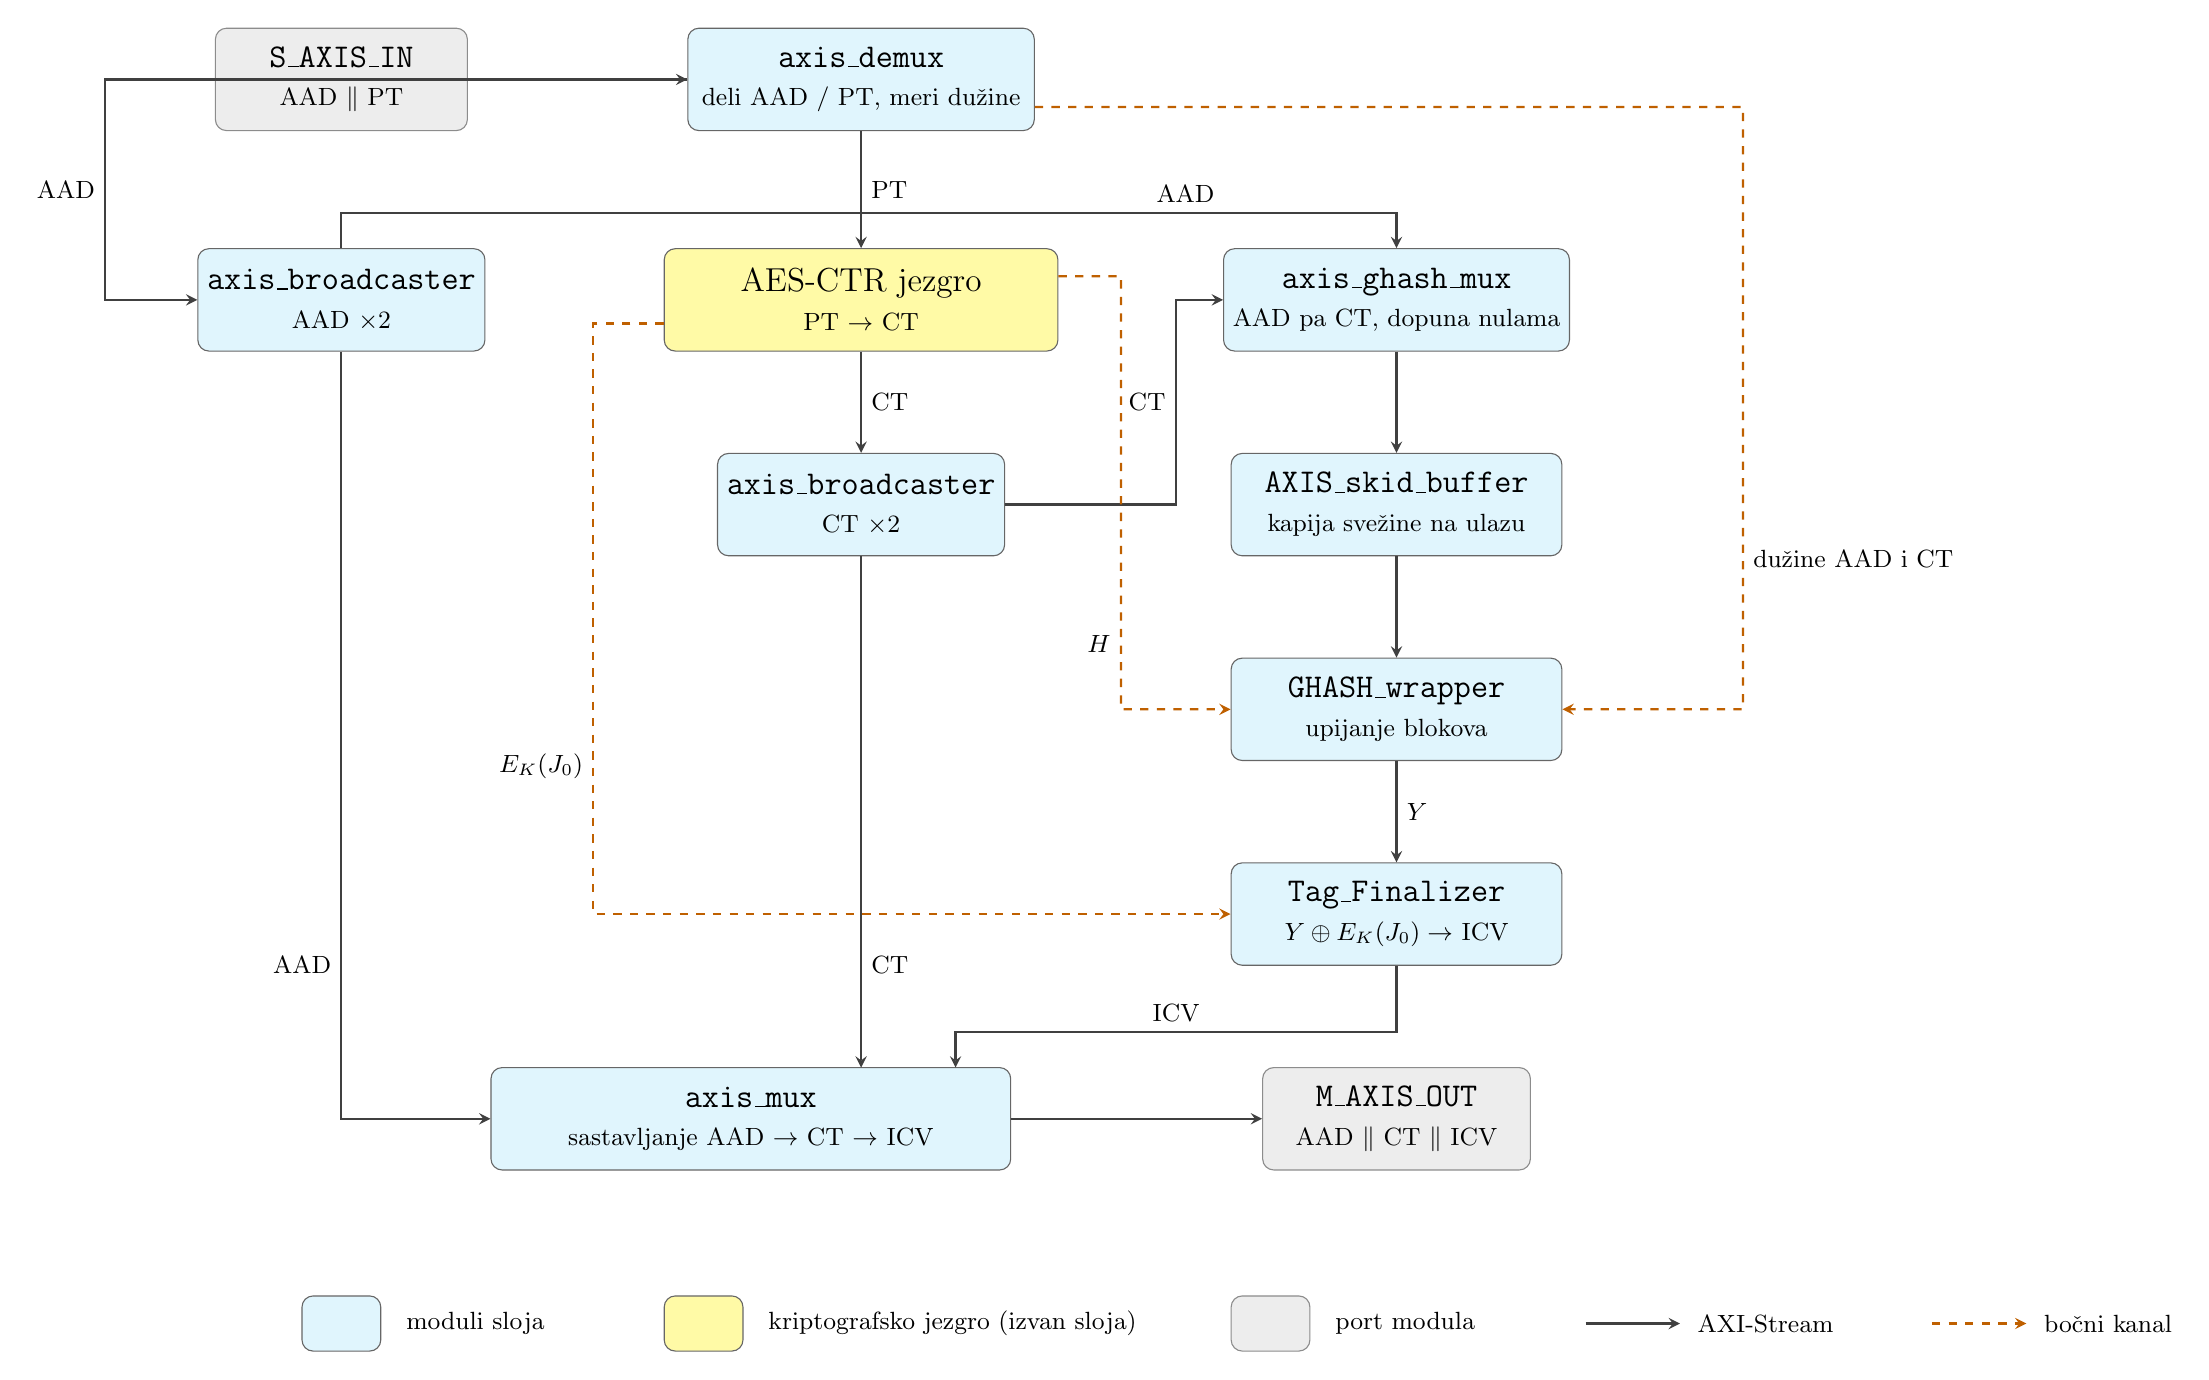
\begin{tikzpicture}[font=\large, >=stealth,
    rtl/.style={rectangle, rounded corners=4pt, draw=black!60, fill=cyan!12,
                minimum height=1.3cm, text centered, align=center},
    port/.style={rectangle, rounded corners=4pt, draw=black!45, fill=gray!14,
                 minimum height=1.3cm, text centered, align=center},
    jezgro/.style={rectangle, rounded corners=4pt, draw=black!60, fill=yellow!35,
                   minimum height=1.3cm, text centered, align=center},
    tok/.style={->, thick, draw=black!75},
    bok/.style={->, thick, dashed, draw=orange!75!black}]

    % ---------------- blokovi ----------------
    \node (in)   [port,   minimum width=3.2cm] at (0,7.4)      {\texttt{S\_AXIS\_IN}\\ {\small AAD $\|$ PT}};
    \node (dmx)  [rtl,    minimum width=4.4cm] at (6.6,7.4)    {\texttt{axis\_demux}\\ {\small deli AAD / PT, meri dužine}};
    \node (bcA)  [rtl,    minimum width=3.6cm] at (0,4.6)      {\texttt{axis\_broadcaster}\\ {\small AAD $\times 2$}};
    \node (aes)  [jezgro, minimum width=5.0cm] at (6.6,4.6)    {AES-CTR jezgro\\ {\small PT $\to$ CT}};
    \node (gmux) [rtl,    minimum width=4.2cm] at (13.4,4.6)   {\texttt{axis\_ghash\_mux}\\ {\small AAD pa CT, dopuna nulama}};
    \node (bcC)  [rtl,    minimum width=3.6cm] at (6.6,2.0)    {\texttt{axis\_broadcaster}\\ {\small CT $\times 2$}};
    \node (skid) [rtl,    minimum width=4.2cm] at (13.4,2.0)   {\texttt{AXIS\_skid\_buffer}\\ {\small kapija svežine na ulazu}};
    \node (gh)   [rtl,    minimum width=4.2cm] at (13.4,-0.6)  {\texttt{GHASH\_wrapper}\\ {\small upijanje blokova}};
    \node (tag)  [rtl,    minimum width=4.2cm] at (13.4,-3.2)  {\texttt{Tag\_Finalizer}\\ {\small $Y \oplus E_K(J_0) \to$ ICV}};
    \node (mux)  [rtl,    minimum width=6.6cm] at (5.2,-5.8)   {\texttt{axis\_mux}\\ {\small sastavljanje AAD $\to$ CT $\to$ ICV}};
    \node (out)  [port,   minimum width=3.4cm] at (13.4,-5.8)  {\texttt{M\_AXIS\_OUT}\\ {\small AAD $\|$ CT $\|$ ICV}};

    % ---------------- tokovi ----------------
    % Trase idu spoljnim kanalima (levo x=-3.0, desno x=17.8) i koridorom y=5.7
    % iznad reda jezgra; AAD grana ka ghash_mux sece PT liniju, ali nijedna
    % linija ne prolazi kroz blok, a natpisi stoje na dugim pravim potezima.
    \draw [tok] (in) -- (dmx);
    \draw [tok] (dmx) -- node[right, font=\small] {PT} (aes);
    \draw [tok] (dmx.west) -- (-3.0,7.4) -- node[left, font=\small] {AAD} (-3.0,4.6) -- (bcA.west);
    \draw [tok] (bcA.north) -- (0,5.7) -- node[above, font=\small, pos=0.8] {AAD} (13.4,5.7) -- (gmux.north);
    \draw [tok] (aes.south) -- node[right, font=\small] {CT} (bcC.north);
    \draw [tok] (bcC.east) -- (10.6,2.0) -- node[left, font=\small] {CT} (10.6,4.6) -- (gmux.west);
    \draw [tok] (gmux) -- (skid);
    \draw [tok] (skid) -- (gh);
    \draw [tok] (gh) -- node[right, font=\small] {$Y$} (tag);
    \draw [tok] (bcA.south) -- node[left, font=\small, pos=0.8] {AAD} (0,-5.8) -- (mux.west);
    \draw [tok] (bcC.south) -- node[right, font=\small, pos=0.8] {CT} (6.6,-5.15);
    \draw [tok] (tag.south) -- (13.4,-4.7) -- node[above, font=\small] {ICV} (7.8,-4.7) -- (7.8,-5.15);
    \draw [tok] (mux) -- (out);

    % ---------------- bocni kanali ----------------
    \draw [bok] ([yshift=0.3cm]aes.east) -- (9.9,4.9) -- node[left, font=\small, pos=0.85] {$H$} (9.9,-0.6) -- (gh.west);
    \draw [bok] ([yshift=-0.3cm]aes.west) -- (3.2,4.3) -- node[left, font=\small, pos=0.75] {$E_K(J_0)$} (3.2,-3.2) -- (tag.west);
    \draw [bok] ([yshift=-0.35cm]dmx.east) -- (17.8,7.05) -- node[right, font=\small, pos=0.75] {dužine AAD i CT} (17.8,-0.6) -- (gh.east);

    % ---------------- legenda ----------------
    \begin{scope}[shift={(0,-8.4)}]
        \node (l1) [rtl,    minimum width=1.0cm, minimum height=0.7cm] at (0,0) {};
        \node [anchor=west, font=\small] at (0.7,0) {moduli sloja};
        \node (l2) [jezgro, minimum width=1.0cm, minimum height=0.7cm] at (4.6,0) {};
        \node [anchor=west, font=\small] at (5.3,0) {kriptografsko jezgro (izvan sloja)};
        \node (l3) [port,   minimum width=1.0cm, minimum height=0.7cm] at (11.8,0) {};
        \node [anchor=west, font=\small] at (12.5,0) {port modula};
        \draw [tok] (15.8,0) -- (17.0,0); \node [anchor=west, font=\small] at (17.1,0) {AXI-Stream};
        \draw [bok] (20.2,0) -- (21.4,0); \node [anchor=west, font=\small] at (21.5,0) {bočni kanal};
    \end{scope}
\end{tikzpicture}
}
\caption{Moduli GCM sloja na putu šifrovanja}
\label{fig:gcm_glue}
\end{figure}

Moduli sa slike, redom kojim podatak putuje kroz sloj:
\smallbreak
\textit{Razdvajanje segmenata} (\texttt{axis\_demux}) deli ulazni tok na AAD i PT. Granica nije označena u samim podacima. Akcelerator štiti pakete unapred poznatog formata, pa je dužina AAD segmenta generik, utvrđen pri sintezi. Dužinu korisnog sadržaja modul meri u hodu, brojeći reči i važeće bajtove poslednje, i obe dužine šalje bočnim kanalom za završni blok GHASH funkcije.
\smallbreak
\textit{Grananje} (\texttt{axis\_broadcaster}) pravi dve istovetne kopije toka, bez sopstvenog skladišta. Reč prolazi tek kada su oba potrošača spremna, pa sporiji od njih zadržava i bržeg. Instancirana su dva, jedan za AAD i jedan za šifrat, u oba slučaja sa po jednom kopijom za autentifikacioni put i jednom za izlaz.
\smallbreak
\textit{Multiplekser autentifikacionog puta} (\texttt{axis\_ghash\_mux}) sastavlja redosled koji GHASH zahteva: najpre svi AAD blokovi, zatim svi blokovi šifrata. Usput sprovodi pravilo dopune iz standarda, tako što bajtove koje maska \texttt{tkeep} ne pokriva postavlja na nulu, pa nepotpun poslednji blok segmenta ulazi u GHASH kao čist 128-bitni koeficijent. Maskiranje važi samo za ovu granu, kopija šifrata koja putuje ka izlazu ostaje netaknuta.
\smallbreak
\textit{Skid bafer} (\texttt{AXIS\_skid\_buffer}) je registarski stepen sa jednim rezervnim mestom, umetnut po pravilu iz odeljka \ref{subsec:hw_axis}. Registruje rukovanje u oba smera i time prekida kombinacionu putanju \texttt{tready} signala na ulazu u GHASH omotač. Rezervno mesto pritom čuva reč zatečenu u letu kada omotač u dvotaktnoj varijanti spusti spremnost. Na njegovom ulazu i kapija svežine iz odeljka \ref{subsec:hw_gcm_kapija} zaustavlja početak novog paketa.
\smallbreak
\textit{GHASH omotač} (\texttt{GHASH\_wrapper}) vodi jedinicu iz odeljka \ref{subsec:hw_ghash}: upija blokove pristigle sa multipleksera, po poslednjem sam dodaje završni blok sa dužinama, sastavljen od vrednosti primljenih od razdvajanja segmenata, i vraća konačan sažetak $Y$. Čita isti generik \texttt{MULT\_CYCLES} kao i jedinica i u dvotaktnoj varijanti spušta spremnost svaki drugi takt. To je modul koji dotok prilagođava ritmu množača, najavljen u odeljku \ref{subsec:hw_ghash_cycles}.
\smallbreak
\textit{Završetak oznake} (\texttt{Tag\_Finalizer}) pamti $E_K(J_0)$ čim ga jezgro izračuna, a kada stigne konačno $Y$, računa $\mathrm{ICV} = Y \oplus E_K(J_0)$ i izdaje oznaku kao jednu reč toka, koju drži dok je izlaz ne preuzme.
\smallbreak
\textit{Sastavljanje izlaza} (\texttt{axis\_mux}) spaja tri toka u izlazni paket utvrđenim redom: AAD, šifrat, oznaka, a \texttt{tlast} podiže tek na reči sa oznakom.

\subsubsection{Prevođenje redosleda bajtova}

Dve konvencije se ovde susreću. AXI4-Stream nosi nulti bajt toka u najnižoj poziciji reči. Pri širini magistrale od 128 bita prvi bajt paketa stiže na linijama $[7{:}0]$, a šesnaesti na $[127{:}120]$. AES i GHASH, nasuprot tome, nulti bajt bloka smeštaju na najvišu poziciju. Bez prevođenja, prvi bajt niza za šifrovanje sabirao bi se sa poslednjim bajtom otvorenog teksta.
\smallbreak
Prevođenje je zato svedeno na tačno dve tačke, ulazni i izlazni port sloja, gde se reč obrće po bajtovima, a maska \texttt{tkeep} po bitovima, tako da preživljava pravilo „bit $i$ označava bajt $i$". Tok podatka kroz te dve tačke prikazan je u tabeli \ref{tab:byte_order}. Time nijedan modul unutar sloja ne mora znati za konvenciju, a nepotpuna poslednja reč prirodno smešta svoje bajtove na najviše pozicije bloka, ostavljajući nule iza njih, što je upravo pravilo dopunjavanja nulama iz GCM standarda.

\begin{table}[H]
\caption{Redosled bajtova kroz akcelerator, na primeru bloka $\mathtt{00\,11\,22\,\ldots\,ff}$}
\centering
\resizebox{\textwidth}{!}{
\begin{tabular}{|c|c|}
\hline
\rowcolor{gray!30}
Tačka u sistemu & Vrednost \\
\hline
u memoriji (redom bajtova) & \texttt{00 11 22 33 44 55 66 77 88 99 aa bb cc dd ee ff} \\
\hline
na \texttt{s\_axis\_tdata[127:0]} & \texttt{ff ee dd cc bb aa 99 88 77 66 55 44 33 22 11 00} \\
\hline
posle obrtanja, kao AES blok & \texttt{00 11 22 33 44 55 66 77 88 99 aa bb cc dd ee ff} \\
\hline
šifrat kao AES blok & \texttt{8a b2 82 15 ee 2f 29 6c ce 92 f7 66 b7 c0 67 c0} \\
\hline
na \texttt{m\_axis\_tdata[127:0]} & \texttt{c0 67 c0 b7 66 f7 92 ce 6c 29 2f ee 15 82 b2 8a} \\
\hline
u memoriji (redom bajtova) & \texttt{8a b2 82 15 ee 2f 29 6c ce 92 f7 66 b7 c0 67 c0} \\
\hline
\end{tabular}
}
\label{tab:byte_order}
\end{table}

Sa prevođenjem na oba porta, prvi bajt niza za šifrovanje sabira se sa prvim bajtom otvorenog teksta, a šifrat koji se vraća u memoriju bajt po bajt jednak je onom koji standard propisuje za iste ulaze.
\smallbreak
Upravo se zato ovo mesto proverava testovima sa poznatim odgovorima, o kojima je reč u odeljku \ref{sec:rez_metodologija}.

\subsubsection{Kapija svežine heš potključa}
\label{subsec:hw_gcm_kapija}

Ova kapija postoji zbog jedne posledice koja se lako previdi. GHASH može da počne rad pre nego što je spreman. Pridruženi podaci ulaze u GHASH pre korisnog sadržaja, a oni ne zavise od šifre, pa sloj nema prirodan razlog da ih zadrži, a na putu dešifrovanja u GHASH ulazi primljeni šifrat, koji kroz jezgro i ne prolazi. Heš potključ $H$, međutim, zavisi od ključa i dobija se tek pošto jezgro izračuna $E_K(0^{128})$. Pri gustom saobraćaju, kada nov ključ stigne uz nov paket, prve reči tog paketa mogu stići pre te vrednosti.
\smallbreak
Posledica bi bila upijanje sa zastarelim $H$, dakle oznaka izračunata pogrešnim potključem. To je greška koja se ne prijavljuje ni na jednoj strani. Pošiljalac bi proizveo oznaku koju primalac odbacuje, a uzrok bi bio vidljiv samo pod gustim saobraćajem i tek na paketu koji nosi promenu ključa.
\smallbreak
Rešenje je jedan bočni signal i jedno pravilo. Jezgro drži signal aktivnim dok $H$ za novi ključ nije preračunat, a sloj dok signal traje zadržava početak novog paketa na ulazu u GHASH. Paket koji već traje kapija nikada i ne presreće, jer ključ pristigao usred paketa čeka u senci do ciklusa pražnjenja (odeljak \ref{subsec:hw_aes_kljuc}), pa se potključ tekućeg paketa ne može promeniti. Kapija, dakle, deluje samo na granici paketa.

\subsubsection{Razlike puta dešifrovanja}

Sloj na putu dešifrovanja zadržava strukturu puta šifrovanja. Grananje, multiplekser autentifikacionog puta, skid bafer i GHASH omotač isti su moduli, samo grananje šifrata sada stoji ispred kriptografske granice, jer standard propisuje da se autentifikuje ono što je primljeno, a ne ono što je dobijeno dešifrovanjem (odeljak \ref{subsubsec:ghash}), pa GHASH radi nad primljenim šifratom, pre XOR-a. Tri modula su drugačija:
\begin{itemize}[itemsep=2pt]
    \item \textit{Razdvajanje segmenata} (\texttt{axis\_demux\_dec}) deli ulazni tok na tri segmenta, jer paket pored AAD i šifrata nosi i oznaku. Pošto je poslednja reč šifrata poznata tek kada stigne oznaka, modul u sopstvenom skid baferu zadržava jednu reč šifrata, da bi \texttt{tlast} pao na stvarno poslednju reč.
    \item \textit{Provera oznake} (\texttt{Tag\_Verifier}) zamenjuje završetak oznake. Izračunatu i primljenu vrednost prihvata bilo kojim redosledom, prva pristigla se pamti dok ne stigne i druga.
    \item \textit{Sastavljanje izlaza} (\texttt{axis\_mux\_dec}) drži poslednju reč otvorenog teksta dok rezultat provere oznake ne bude poznat, pa je zatim šalje zajedno sa \texttt{tlast} i signalom ispravnosti. Potrošač tako saznaje da li je paket autentičan u istom taktu u kome prima njegov poslednji bajt, i može ga odbaciti, čime se poštuje pravilo iz odeljka \ref{subsubsec:ghash} da dešifrovani sadržaj ne sme biti prosleđen dalje pre uspešne provere.
\end{itemize}
Kompletan raspored modula dat je na slici \ref{fig:gcm_glue_dec}.

\begin{figure}[H]
\centering
\resizebox{\textwidth}{!}{
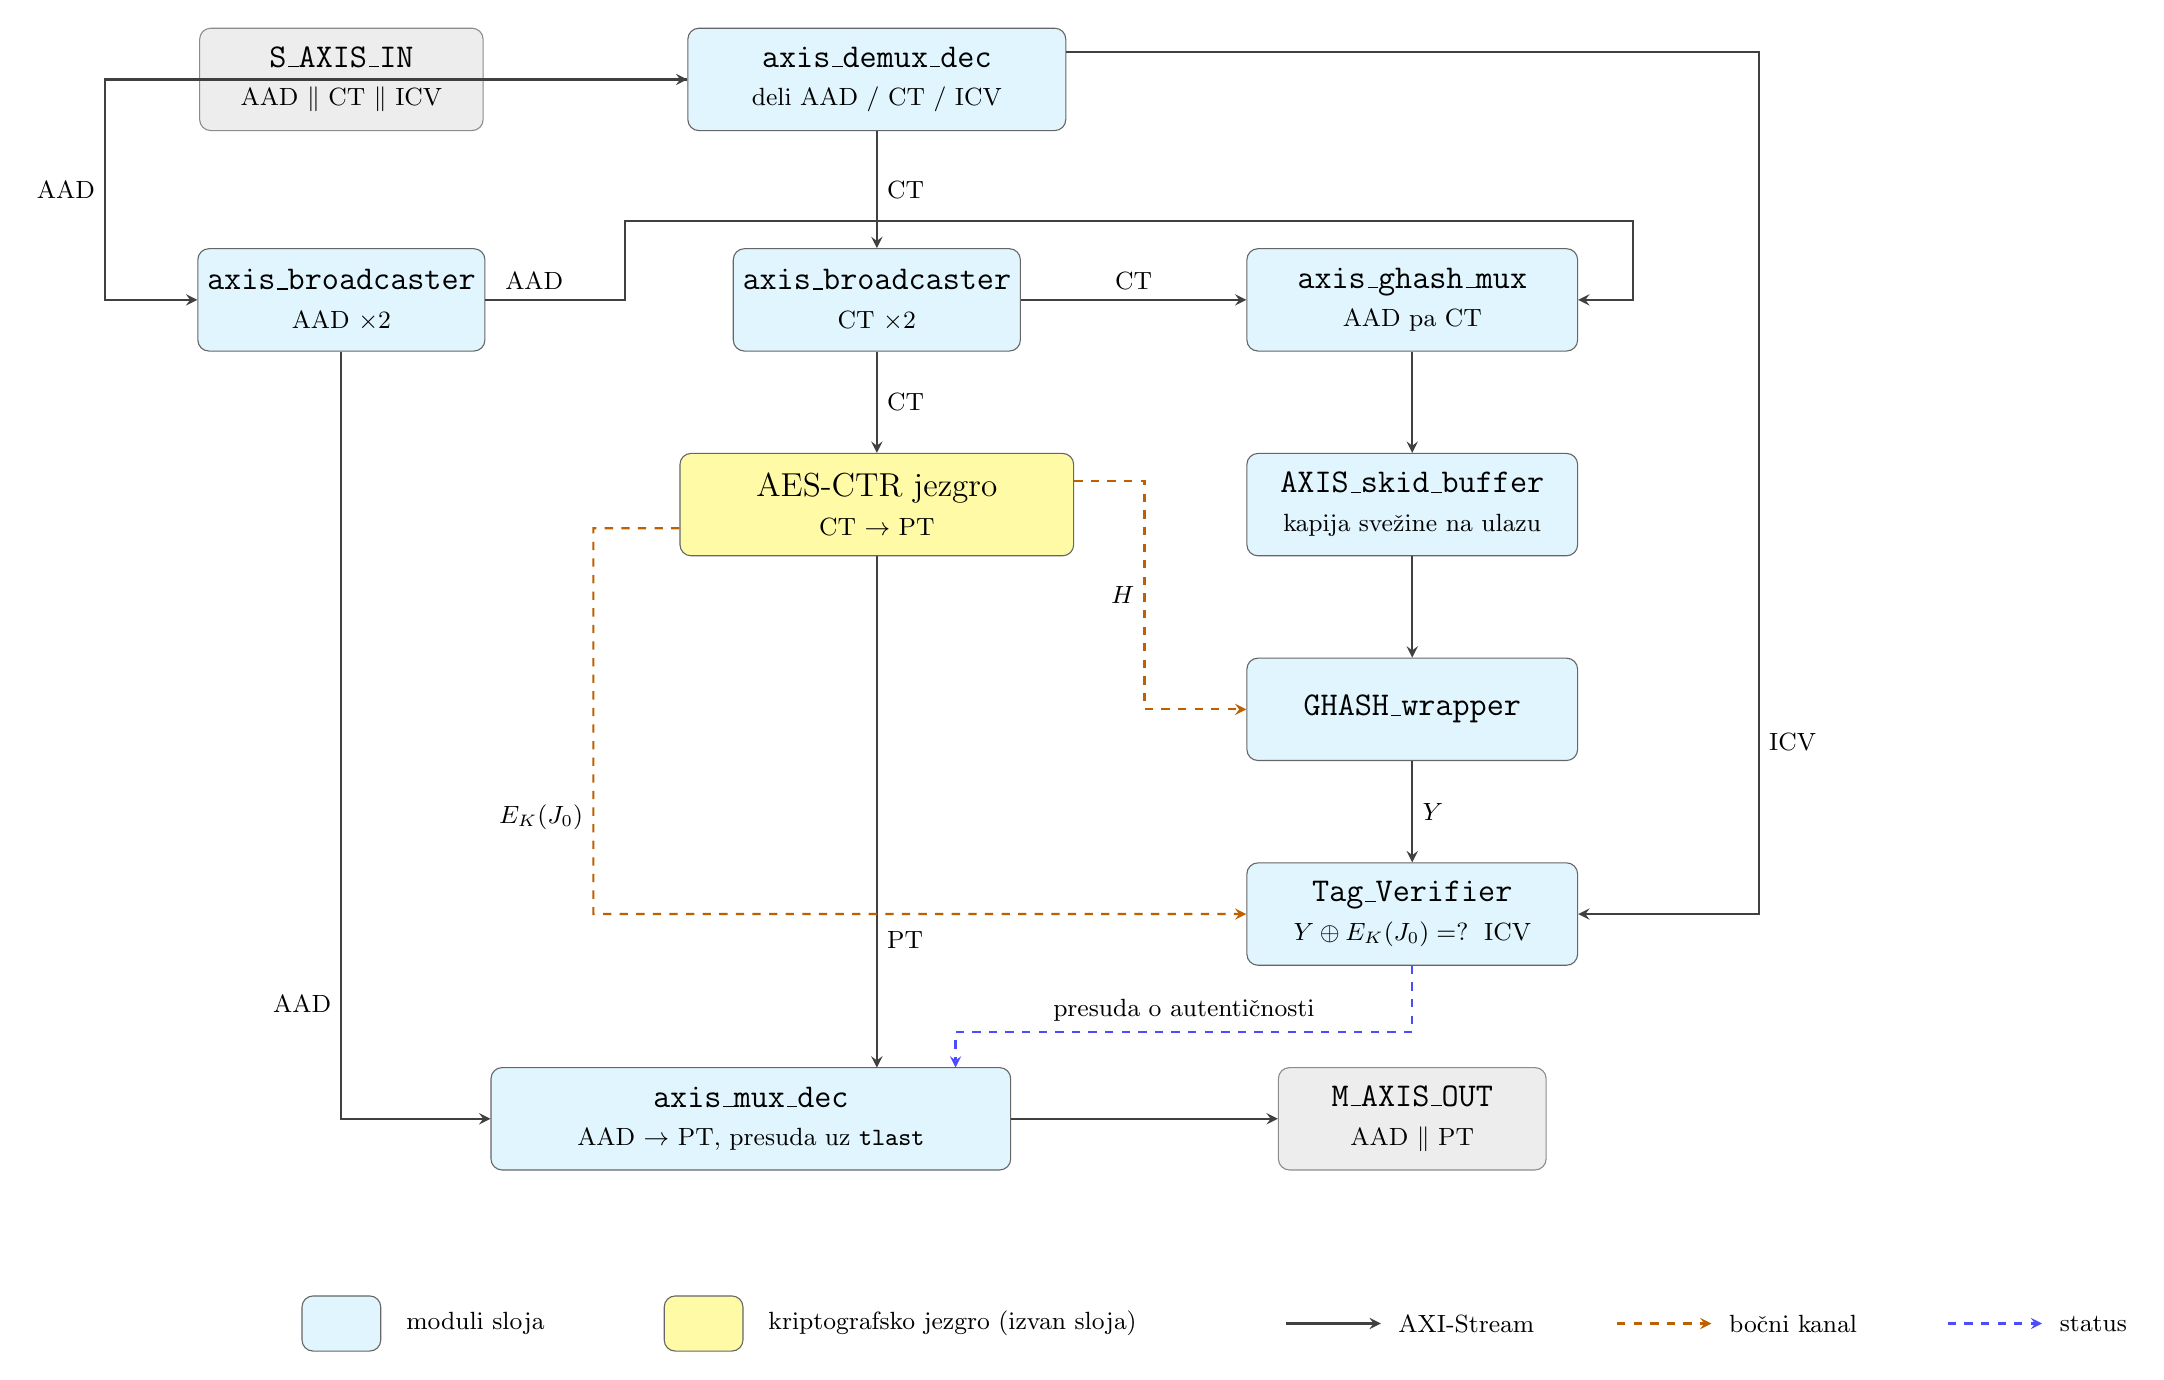
\begin{tikzpicture}[font=\large, >=stealth,
    rtl/.style={rectangle, rounded corners=4pt, draw=black!60, fill=cyan!12,
                minimum height=1.3cm, text centered, align=center},
    port/.style={rectangle, rounded corners=4pt, draw=black!45, fill=gray!14,
                 minimum height=1.3cm, text centered, align=center},
    jezgro/.style={rectangle, rounded corners=4pt, draw=black!60, fill=yellow!35,
                   minimum height=1.3cm, text centered, align=center},
    tok/.style={->, thick, draw=black!75},
    bok/.style={->, thick, dashed, draw=orange!75!black},
    stat/.style={->, thick, dashed, draw=blue!70}]

    \node (in)   [port,   minimum width=3.6cm] at (0,7.4)      {\texttt{S\_AXIS\_IN}\\ {\small AAD $\|$ CT $\|$ ICV}};
    \node (dmx)  [rtl,    minimum width=4.8cm] at (6.8,7.4)    {\texttt{axis\_demux\_dec}\\ {\small deli AAD / CT / ICV}};
    \node (bcA)  [rtl,    minimum width=3.6cm] at (0,4.6)      {\texttt{axis\_broadcaster}\\ {\small AAD $\times 2$}};
    \node (bcC)  [rtl,    minimum width=3.6cm] at (6.8,4.6)    {\texttt{axis\_broadcaster}\\ {\small CT $\times 2$}};
    \node (gmux) [rtl,    minimum width=4.2cm] at (13.6,4.6)   {\texttt{axis\_ghash\_mux}\\ {\small AAD pa CT}};
    \node (aes)  [jezgro, minimum width=5.0cm] at (6.8,2.0)    {AES-CTR jezgro\\ {\small CT $\to$ PT}};
    \node (skid) [rtl,    minimum width=4.2cm] at (13.6,2.0)   {\texttt{AXIS\_skid\_buffer}\\ {\small kapija svežine na ulazu}};
    \node (gh)   [rtl,    minimum width=4.2cm] at (13.6,-0.6)  {\texttt{GHASH\_wrapper}};
    \node (ver)  [rtl,    minimum width=4.2cm] at (13.6,-3.2)  {\texttt{Tag\_Verifier}\\ {\small $Y \oplus E_K(J_0) \;{=}?\; $ ICV}};
    \node (mux)  [rtl,    minimum width=6.6cm] at (5.2,-5.8)   {\texttt{axis\_mux\_dec}\\ {\small AAD $\to$ PT, presuda uz \texttt{tlast}}};
    \node (out)  [port,   minimum width=3.4cm] at (13.6,-5.8)  {\texttt{M\_AXIS\_OUT}\\ {\small AAD $\|$ PT}};

    % tokovi
    \draw [tok] (in) -- (dmx);
    \draw [tok] (dmx) -- node[right, font=\small] {CT} (bcC);
    \draw [tok] (dmx.west) -- (-3.0,7.4) -- node[left, font=\small] {AAD} (-3.0,4.6) -- (bcA.west);
    \draw [tok] (bcC.east) -- node[above, font=\small] {CT} (gmux.west);
    \draw [tok] (bcA.east) -- node[above, font=\small, pos=0.35] {AAD} (3.6,4.6) -- (3.6,5.6) -- (16.4,5.6) -- (16.4,4.6) -- (gmux.east);
    \draw [tok] (bcC.south) -- node[right, font=\small] {CT} (aes.north);
    \draw [tok] (gmux) -- (skid);
    \draw [tok] (skid) -- (gh);
    \draw [tok] (gh) -- node[right, font=\small] {$Y$} (ver);
    \draw [tok] (bcA.south) -- node[left, font=\small, pos=0.85] {AAD} (0,-5.8) -- (mux.west);
    \draw [tok] (aes.south) -- node[right, font=\small, pos=0.75] {PT} (6.8,-5.15);
    \draw [tok] ([yshift=0.35cm]dmx.east) -- (18.0,7.75) -- node[right, font=\small, pos=0.8] {ICV} (18.0,-3.2) -- (ver.east);

    % bocni kanali i status
    \draw [bok] ([yshift=0.3cm]aes.east) -- (10.2,2.3) -- node[left, font=\small] {$H$} (10.2,-0.6) -- (gh.west);
    \draw [bok] ([yshift=-0.3cm]aes.west) -- (3.2,1.7) -- node[left, font=\small, pos=0.75] {$E_K(J_0)$} (3.2,-3.2) -- (ver.west);
    \draw [stat] (ver.south) -- (13.6,-4.7) -- node[above, font=\small] {presuda o autentičnosti} (7.8,-4.7) -- (7.8,-5.15);
    \draw [tok] (mux) -- (out);

    % legenda
    \begin{scope}[shift={(0,-8.4)}]
        \node [rtl,    minimum width=1.0cm, minimum height=0.7cm] at (0,0) {};
        \node [anchor=west, font=\small] at (0.7,0) {moduli sloja};
        \node [jezgro, minimum width=1.0cm, minimum height=0.7cm] at (4.6,0) {};
        \node [anchor=west, font=\small] at (5.3,0) {kriptografsko jezgro (izvan sloja)};
        \draw [tok]  (12.0,0) -- (13.2,0); \node [anchor=west, font=\small] at (13.3,0) {AXI-Stream};
        \draw [bok]  (16.2,0) -- (17.4,0); \node [anchor=west, font=\small] at (17.5,0) {bočni kanal};
        \draw [stat] (20.4,0) -- (21.6,0); \node [anchor=west, font=\small] at (21.7,0) {status};
    \end{scope}
\end{tikzpicture}
}
\caption{Moduli GCM sloja na putu dešifrovanja}
\label{fig:gcm_glue_dec}
\end{figure}

\subsection{Sistemski omotač}
\label{subsec:hw_l3}

Do sada opisani deo akceleratora radi sa već razdvojenim segmentima. Stvaran paket, međutim, stiže kao jedan neprekidan niz bajtova u kome granice segmenata nisu ničim označene, i po pravilu ne padaju na granicu reči magistrale. Ako je zaglavlje koje se prenosi nepromenjeno dugačko 34 bajta, a magistrala široka 16, treća reč paketa sadrži i poslednja dva bajta zaglavlja i prvih četrnaest bajtova pridruženih podataka. Sistemski omotač rešava upravo taj problem. U osnovi ga čini par jezgara, razdvajanje i sastavljanje, uz skid bafere između njih i, na putu dešifrovanja, jezgro za poravnanje oznake.
\smallbreak
\textit{Razdvajanje} (SPLIT) deli ulazni tok na dva izlaza: segment koji se prenosi nepromenjen i ostatak, pri čemu svaki segment mora početi od nultog bajta svoje reči, jer to GCM sloj očekuje. Pošto granice padaju usred reči, modul sadrži prenosni registar (engl. \textit{gearbox}), koji zadržava bajtove narednog segmenta pristigle u graničnoj reči i poravnava ih uz sledeće.
\smallbreak
\textit{Sastavljanje} (MERGE) je inverzna operacija. Od dva toka pravi jedan neprekidan, tako da je samo poslednja reč nepotpuna. Vredi uočiti asimetriju. Sastavljanju nije potreban nijedan generik sa dužinom, jer oba ulazna toka sama najavljuju svoj kraj signalom \texttt{tlast}. Razdvajanju jeste, jer ono mora da preseče jedan tok na mestu koje u podacima ništa ne označava.
\smallbreak
Uz njih idu i skid baferi, tri na putu šifrovanja i četiri na putu dešifrovanja, na samom ulazu, na izlazu, na grani BYPASS i, pri dešifrovanju, na kriptografskoj grani pred poravnanjem oznake. Svaki registruje rukovanje u oba smera i time prekida kombinacione putanje između jezgara. Razdvajanje i sastavljanje imaju i generik kojim se segment BYPASS isključuje u potpunosti, za pakete koji počinju neposredno pridruženim podacima. Razdvajanje tada kreće od segmenta AAD, sastavljanje samo prosleđuje kriptografski tok, a portovi kojima segment BYPASS putuje i skid bafer između njih nestaju iz sistema. Lanac na putu šifrovanja prikazan je na slici \ref{fig:l3_lanac}.

\begin{figure}[H]
\centering
\resizebox{\textwidth}{!}{
\begin{tikzpicture}[font=\large]
    % Dve grane su vodoravne i razmaknute po visini, pa natpisi stoje uspravno
    % iznad odnosno ispod svoje strelice i ne prelaze ni preko linija ni preko blokova.
    \def\yb{1.9}\def\yg{-1.9}
    \node (in)  [blokdata,     minimum width=2.2cm, minimum height=1.2cm, align=center] at (0,0)      {paket\\ (AXIS)};
    \node (sp)  [blokkripto,   minimum width=2.6cm, minimum height=1.2cm, align=center] at (3.4,0)    {razdvajanje\\ (SPLIT)};
    \node (byp) [blokdata,     minimum width=4.6cm, minimum height=1.2cm, align=center] at (9.0,\yb)  {nepromenjeni segment};
    \node (gcm) [blokghash,    minimum width=4.6cm, minimum height=1.2cm, align=center] at (9.0,\yg)  {GCM sloj {\small +} jezgro};
    \node (mg)  [blokkripto,   minimum width=2.6cm, minimum height=1.2cm, align=center] at (14.6,0)   {sastavljanje\\ (MERGE)};
    \node (out) [blokrezultat, minimum width=2.2cm, minimum height=1.2cm, align=center] at (18.0,0)   {paket\\ (AXIS)};

    \draw [strelica] (in) -- (sp);
    % Natpisi su zasebni cvorovi na praznim delovima, jer bi pos= na izlomljenoj
    % putanji merio duz cele duzine i sleteo na ivicu bloka.
    % gornja grana
    \draw [strelica] ([yshift=0.3cm]sp.east) -- (5.9,0.3) -- (5.9,\yb) -- (byp.west);
    \draw [strelica] (byp.east) -- (12.9,\yb) -- (12.9,0.3) -- ([yshift=0.3cm]mg.west);
    \node [font=\small, anchor=east] at (5.6,1.05) {BYPASS};
    % donja grana
    \draw [strelica] ([yshift=-0.3cm]sp.east) -- (5.9,-0.3) -- (5.9,\yg) -- (gcm.west);
    \draw [strelica] (gcm.east) -- (12.9,\yg) -- (12.9,-0.3) -- ([yshift=-0.3cm]mg.west);
    \node [font=\small, anchor=east] at (5.6,-1.05) {AAD $\|$ PT};
    \node [font=\small, anchor=west] at (13.2,-1.05) {AAD $\|$ CT $\|$ ICV};
    \draw [strelica] (mg) -- (out);
\end{tikzpicture}
}
\caption{Sistemski omotač na putu šifrovanja}
\label{fig:l3_lanac}
\end{figure}

Na strani dešifrovanja lanac ima jedno jezgro više, i to zbog razlike koja postoji samo u tom smeru. Pri šifrovanju oznaka nastaje unutar GCM sloja, koji je sam stavlja na kraj. Pri dešifrovanju oznaka stiže spolja, spakovana neposredno uz šifrat. Pošto dužina korisnog sadržaja nije unapred poznata, poslednjih šesnaest bajtova paketa je oznaka, a kako se njen početak najčešće zatekne usred reči, njeni bajtovi su razdeljeni na poslednje dve reči. GCM sloj, međutim, zahteva oznaku samu na poslednjoj reči.
\smallbreak
Taj razmak popunjava jezgro \texttt{ICV\_realign}. Ono zadržava po jednu reč unazad, jer se tek sa signalom \texttt{tlast} sazna koliko bajtova poslednje reči pripada oznaci. Ako je $k$ broj važećih bajtova u poslednjoj reči, rep šifrata su donjih $k$ bajtova zapamćene reči, a oznaka se sastavlja od preostalih bajtova te reči i bajtova poslednje.
\smallbreak
Bitno je uočiti da se pri tome ništa ne dodaje. Broj reči ostaje isti, kao i broj važećih bajtova. Jedino se praznina, koja je pre preuređenja stajala u poslednjoj reči iza oznake, premešta u pretposlednju, iza repa šifrata. Rezultat je tok u kome poslednja reč šifrata sme biti nepotpuna, a oznaka zauzima celu narednu reč, sa \texttt{tlast} na njoj. Postupak je, na primeru repa šifrata od četiri bajta, prikazan na slici \ref{fig:l3_lanac_dec}.

\begin{figure}[H]
\centering
\resizebox{\textwidth}{!}{
\begin{tikzpicture}[font=\large, >=stealth]
    % ---------------- lanac ----------------
    \def\yb{2.0}\def\yg{-2.0}
    \node (in)  [blokdata,     minimum width=2.2cm, minimum height=1.2cm, align=center] at (0,0)     {paket\\ (AXIS)};
    \node (sp)  [blokkripto,   minimum width=2.6cm, minimum height=1.2cm, align=center] at (3.4,0)   {razdvajanje\\ (SPLIT)};
    \node (byp) [blokdata,     minimum width=4.6cm, minimum height=1.2cm, align=center] at (9.4,\yb) {nepromenjeni segment};
    \node (icv) [blokrezultat, minimum width=3.4cm, minimum height=1.2cm, align=center] at (8.0,\yg) {\texttt{ICV\_realign}};
    \node (gcm) [blokghash,    minimum width=4.2cm, minimum height=1.2cm, align=center] at (15.2,\yg){GCM sloj {\small +} jezgro};
    \node (mg)  [blokkripto,   minimum width=2.6cm, minimum height=1.2cm, align=center] at (20.0,0)  {sastavljanje\\ (MERGE)};
    \node (out) [blokdata,     minimum width=2.2cm, minimum height=1.2cm, align=center] at (23.4,0)  {paket\\ (AXIS)};

    \draw [strelica] (in) -- (sp);
    \draw [strelica] ([yshift=0.3cm]sp.east) -- (5.9,0.3) -- (5.9,\yb) -- (byp.west);
    \draw [strelica] (byp.east) -- (18.3,\yb) -- (18.3,0.3) -- ([yshift=0.3cm]mg.west);
    \node [font=\small, anchor=east] at (5.6,1.1) {BYPASS};
    \draw [strelica] ([yshift=-0.3cm]sp.east) -- (5.9,-0.3) -- (5.9,\yg) -- (icv.west);
    \node [font=\small, anchor=east] at (5.6,-1.1) {AAD $\|$ CT $\|$ ICV};
    \draw [strelica] (icv) -- node[above, font=\small] {ICV zasebno} (gcm.west);
    \draw [strelica] (gcm.east) -- (18.3,\yg) -- (18.3,-0.3) -- ([yshift=-0.3cm]mg.west);
    \node [font=\small, anchor=west] at (18.6,-1.1) {AAD $\|$ PT};
    \draw [strelica] (mg) -- (out);

    % ---------------- rasporedjivanje reci ----------------
    % Primer: magistrala 16 B po reci, rep sifrata k = 4 B, oznaka 16 B.
    % Ukupno 36 B, dakle tri reci u oba slucaja; preuredjenjem se ne dodaje
    % nijedan bajt, nego se praznina samo premesta iz poslednje reci u pretposlednju.
    \begin{scope}[shift={(0,-7.2)}, every node/.style={font=\small}]
        \def\W{4.0}\def\G{0.45}
        \def\xA{0}\def\xB{4.45}\def\xC{8.9}

        \node [anchor=east, font=\large] at (-0.5,0.55)  {pre};
        \node [anchor=east, font=\large] at (-0.5,-1.95) {posle};

        % Raspored unutar reci prati AXI4-Stream: bajt 0 je na tdata[7:0], dakle
        % KRAJNJE DESNO, a visi bajtovi levo. Zato dopuna nepotpune reci stoji
        % levo, sto se poklapa sa tim da tkeep pokriva donje bajtove.
        \node [font=\footnotesize, gray!55!black, anchor=south west] at (\xA,1.3)
              {\textleftarrow\ viši bajtovi \hspace{2.2cm} bajt 0 na \texttt{tdata[7:0]} \textrightarrow};

        % ---- PRE ----
        \draw [draw=black!60, fill=cyan!15] (\xA,0) rectangle (\xA+\W,1.1);
        \node at (\xA+2.0,0.55) {CT (16 B)};
        \draw [draw=black!60, fill=red!25]  (\xB,0) rectangle (\xB+3.0,1.1);
        \draw [draw=black!60, fill=cyan!15] (\xB+3.0,0) rectangle (\xB+\W,1.1);
        \node at (\xB+1.5,0.55) {ICV (12 B)};
        \node [font=\footnotesize] at (\xB+3.5,0.55) {CT};
        \draw [draw=black!35, fill=gray!10, dashed] (\xC,0) rectangle (\xC+3.0,1.1);
        \draw [draw=black!60, fill=red!25]  (\xC+3.0,0) rectangle (\xC+\W,1.1);
        \node [gray!55!black] at (\xC+1.5,0.55) {prazno (12 B)};
        \node [font=\footnotesize] at (\xC+3.5,0.55) {ICV};
        \node [anchor=west] at (\xC+\W+0.5,0.55) {\texttt{tlast}, \texttt{tkeep} $= 4$ B};

        % ---- POSLE ----
        \draw [draw=black!60, fill=cyan!15] (\xA,-2.5) rectangle (\xA+\W,-1.4);
        \node at (\xA+2.0,-1.95) {CT (16 B)};
        \draw [draw=black!35, fill=gray!10, dashed] (\xB,-2.5) rectangle (\xB+3.0,-1.4);
        \draw [draw=black!60, fill=cyan!15] (\xB+3.0,-2.5) rectangle (\xB+\W,-1.4);
        \node [gray!55!black] at (\xB+1.5,-1.95) {prazno (12 B)};
        \node [font=\footnotesize] at (\xB+3.5,-1.95) {CT};
        \node [anchor=north, font=\footnotesize] at (\xB+3.5,-2.6) {\texttt{tkeep} $= 4$ B};
        \draw [draw=black!60, fill=red!25]  (\xC,-2.5) rectangle (\xC+\W,-1.4);
        \node at (\xC+2.0,-1.95) {ICV (16 B)};
        \node [anchor=west] at (\xC+\W+0.5,-1.95) {\texttt{tlast}, cela reč};

        % ---- strelice preuredjenja ----
        \draw [strelica, thick, red!65] (\xB+1.5,0) -- (\xC+1.4,-1.4);
        \draw [strelica, thick, red!65] (\xC+3.5,0) -- (\xC+3.4,-1.4);
        \node [anchor=east, font=\small, red!55!black] at (\xB+1.25,-0.7) {oznaka se sastavlja iz dve reči};

        \node [anchor=north, gray!55!black, font=\small] at (\xB+2.0,-3.3)
              {broj reči je isti, a praznina se samo premešta iz poslednje reči u pretposlednju};
    \end{scope}
\end{tikzpicture}
}
\caption{Sistemski omotač na putu dešifrovanja}
\label{fig:l3_lanac_dec}
\end{figure}

Ovakva organizacija ostvaruje ulogu umetnute zaštite paketa sa početka odeljka. Zaglavlja nižih slojeva prolaze netaknuta, a zaštita se primenjuje tačno na deo paketa koji joj pripada.

\subsection{Pogodnost za dinamičku rekonfiguraciju}
\label{subsec:hw_dfx}

Podela na slojeve iz odeljka \ref{subsec:hw_gcm_pregled} ima posledicu koja prevazilazi urednost opisa. Kriptografska granica, lista portova između sloja i jezgra, nema nijedan signal svojstven AES-u, nego samo ključ, nonce, dva toka podataka i četiri bočna kanala ($H$, maska oznake i dve zastavice stanja). Sve što je vezano za GCM režim (GHASH, blok sa dužinama, oznaka, redosled bajtova, segmenti) stoji sa jedne strane te granice, a sve što je vezano za šifru sa druge.
\smallbreak
Iz toga sledi da je akcelerator prirodno podeljen na \textit{statički deo}, koji se ne menja, i \textit{dinamički deo}, samo jezgro šifre. Takva podela je upravo ono što traži dinamička delimična rekonfiguracija (engl. \textit{Dynamic Function eXchange}, DFX). Particija ima nepromenljiv interfejs, jasno definisan protokol na njemu i nema skrivenog stanja koje bi prelazilo granicu. Zamena algoritma u radu, ili čak zamena jezgra iste šifre drugom arhitekturom, na primer prelazak sa višejezgarne na protočnu prema trenutnom opterećenju, ne zahteva izmenu ostatka sistema.
\smallbreak
Dva ograničenja ipak postoje. Prvo, sadašnji interfejs pretpostavlja da algoritam sam formira brojački blok iz 96-bitne nonce vrednosti. Algoritam koji zahteva drugačiju konstrukciju (recimo pun inicijalizacioni vektor koji generiše neki drugi deo sistema, ili nonce druge dužine) tražio bi manju izmenu granice. Drugo, ključni port je širine 256 bita, pa bi šifra sa dužim ključem takođe zahtevala proširenje. Oba su proširenja same liste portova, ne i logike sa obe strane.

\subsection{Uklapanje u sistem i provera}
\label{subsec:hw_aes_uklapanje}

Za razliku od SHA-3 jezgra, AES-GCM akcelerator stoji u samom mrežnom putu, kao umetnuta zaštita paketa iz odeljka \ref{subsec:hw_gcm_pregled}. Merilo takvog jezgra je propusnost u ustaljenom stanju uz proizvoljan protivpritisak, a ne trajanje pojedinačnog poziva, pa je i celokupno upravljanje tokom podređeno tome.
\smallbreak
Jezgro je provereno na tri nivoa, od vektora sa poznatim odgovorima do rada u postojećem mrežnom sistemu. Postupci i svi rezultati dati su u odeljku \ref{sec:rez_aes}.

\section{Integracija jezgara u lanac}
\label{sec:hw_integracija}

Tri jezgra projektovana su da sarađuju onako kako to nalaže hibridni protokol iz odeljka \ref{sec:hibridni_sistem}, pri čemu SHA-3 jezgro ključ sesije $K$ iz tajne $Z$ izvodi u cSHAKE režimu. Pri tom povezivanju $Z$ i $K$ putuju isključivo između jezgara, unutar programabilne logike, i ni u jednom trenutku ne prolaze kroz memoriju procesorskog sistema. Ciljna organizacija lanca prikazana je na slici \ref{fig:hw_lanac}.
\smallbreak
Ovde se vidi i zašto KMAC nema svoje jezgro. Kako je pokazano u odeljku \ref{subsec:kmac}, KMAC je cSHAKE sa propisanim uokvirivanjem ulaza. Pri tome su svi delovi okvira javni (prefiksni blok, so i kontekst razmene), osim same tajne $Z$. Zato okvir sklapa upravljačka logika ispred SHA-3 jezgra. Javne delove primi unapred pripremljene, a $Z$ umeće neposredno sa tajnog izlaznog toka ECDH jezgra, koji za tu namenu i postoji. Upravo ta podela čini tvrdnju iz prethodnog pasusa ostvarivom, jer strana koja priprema javne delove okvira tajnu nikada ne vidi.
\smallbreak
Upravljačka logika okvira u ovom radu nije realizovana kao zasebno jezgro, pa se ceo lanac sa slike ne sklapa na ploči. Zajednički rad jezgara proverava se simulacijom nad povezanim jezgrima, u kojoj verifikaciono okruženje preuzima upravo tu ulogu: formira KMAC okvir, predaje nonce vrednosti i pokreće jezgra propisanim redosledom. Time se proverava ono što pojedinačni testovi po prirodi ne mogu, a to je da se izlaz jednog jezgra bez izmene prihvata na ulazu narednog. Rezultati su dati u odeljku \ref{sec:rez_sinteza}, a realizacija upravljačke logike kao gotovog IP jezgra spada u nadogradnje o kojima je reč u poglavlju \ref{ch:unapredjenja}.

\begin{figure}[H]
\centering
\resizebox{\textwidth}{!}{
\begin{tikzpicture}[
    sw/.style={rectangle, rounded corners, minimum width=4.6cm, minimum height=1.1cm, align=center, draw=black, fill=gray!20},
    tajna/.style={thick,->,>=stealth,red!70!black}]
    % PL jezgra
    \node (ecdh)   [blokkripto, minimum width=3.2cm, minimum height=1.1cm] at (0,2.4) {ECDH};
    \node (framer) [rectangle, rounded corners, draw=black, fill=gray!35, minimum width=3.6cm, minimum height=1.1cm, align=center] at (0,0) {upravljačka\\ logika okvira};
    \node (sha3)   [blokkripto, minimum width=3.2cm, minimum height=1.1cm, align=center] at (6.2,0) {SHA-3\\ (cSHAKE)};
    \node (aes)    [blokkripto, minimum width=3.2cm, minimum height=1.1cm] at (12.0,0) {AES-GCM};
    \node (pt)     [blokdata, minimum width=3.2cm] at (12.0,2.4) {saobraćaj $\mathrm{PT}$};
    \node (ct)     [blokrezultat, minimum width=3.6cm] at (16.8,0) {$\mathrm{CT} \,\|\, \mathrm{ICV}$};
    % PS strana
    \node (sw1) [sw] at (-7.4,2.4) {javni ključevi razmene};
    \node (sw2) [sw] at (-7.4,0)   {javni delovi okvira\\ (prefiksni blok, so, kontekst)};
    \node (nonce) [rectangle, rounded corners, draw=black, fill=gray!35, minimum width=3.6cm, minimum height=1.1cm, align=center] at (6.2,-2.2) {dodela nonce\\ vrednosti};
    % granica PS/PL
    \draw [dashed, thick, black!60] (-3.9,-3.0) -- (-3.9,3.4);
    \node [anchor=south east, font=\small\itshape] at (-4.0,3.4) {procesorski sistem};
    \node [anchor=south west, font=\small\itshape] at (-3.8,3.4) {programabilna logika};
    % veze
    \draw [strelica, <->] (sw1) -- (ecdh);
    \draw [strelica] (sw2) -- (framer);
    \draw [tajna] (ecdh) -- node[right, font=\small] {tajna $Z$} (framer);
    \draw [strelica] (framer) -- node[above, font=\small] {KMAC okvir} (sha3);
    \draw [tajna] (sha3) -- node[above, font=\small] {ključ $K$} (aes);
    \draw [strelica] (nonce.east) -- (12.0,-2.2) -- (aes.south);
    \draw [strelica] (pt) -- (aes);
    \draw [strelica] (aes) -- (ct);
\end{tikzpicture}
}
\caption[Ciljna organizacija lanca izvođenja i upotrebe ključa]{Ciljna organizacija lanca izvođenja i upotrebe ključa unutar programabilne logike. Crvene strelice nose tajni materijal}
\label{fig:hw_lanac}
\end{figure}

